% Informe final. Compilar main.tex junto con figuras/ mediante pdfLaTeX (dos pasadas) o Tectonic.
\documentclass[11pt,letterpaper]{article}
\usepackage{iftex}
\ifPDFTeX\usepackage[utf8]{inputenc}\fi
\usepackage[T1]{fontenc}
\usepackage[spanish,es-tabla]{babel}
\decimalpoint
\usepackage{lmodern}
\usepackage[margin=2.5cm]{geometry}
\usepackage{microtype}
\usepackage{setspace}
\usepackage{amsmath}
\usepackage{booktabs,tabularx,longtable,array}
\usepackage{enumitem}
\usepackage{graphicx}
\graphicspath{{figuras/}}
\usepackage{placeins}
\usepackage{xurl}
\usepackage[hidelinks]{hyperref}
\hypersetup{pdftitle={Arquitectura modular basada en capacidades: informe final},pdfauthor={Julián Mauricio Ferreira Velásquez}}
\onehalfspacing
\setlength{\emergencystretch}{3em}
\setlength{\parskip}{0.35em}
\setlist{itemsep=0.15em,topsep=0.3em}
\newcolumntype{Y}{>{\raggedright\arraybackslash}X}
\newcolumntype{P}[1]{>{\raggedright\arraybackslash}p{#1}}
\newcommand{\code}[1]{\nolinkurl{#1}}

\begin{document}
\hypersetup{pageanchor=false}
\begin{titlepage}
\centering
{\Large Universidad de los Andes\par}
Departamento de Ingeniería de Sistemas y Computación\par
\vspace{2cm}
{\LARGE\bfseries Arquitectura modular basada en capacidades para la portabilidad de aplicaciones de interacción humano-robot sobre ROS~2\par}
\vspace{1.2cm}
{\Large Proyecto de grado: informe final\par}
\vspace{1.5cm}
{\large Julián Mauricio Ferreira Velásquez\par}
Código: 202012068\par
\vspace{1cm}
Asesor\par
{\large Mario Fernando De la Rosa Rosero\par}
\vfill
Bogotá, Colombia\par
18 de noviembre de 2026\par
\end{titlepage}

\pagenumbering{roman}
\hypersetup{pageanchor=true}
\tableofcontents
\clearpage
\listoffigures
\listoftables
\clearpage
\pagenumbering{arabic}
\setcounter{section}{-1}

\section{Resumen}
Una aplicación que sigue a una persona necesita detectar a quién seguir, decidir cómo moverse y responder cuando se le pide detenerse. Si la aplicación invoca directamente la cámara, el micrófono o la base de un robot, llevar ese comportamiento a otra plataforma obliga a revisar la lógica de interacción. Este proyecto implementó una arquitectura sobre ROS~2 en la que la aplicación consume contratos comunes, Capabilities2 administra sus proveedores y una máquina de estados YASMIN coordina la interacción.

El desarrollo se evaluó en dos etapas. Primero se ejecutaron voz, detección de personas y desplazamiento relativo como funciones individuales en NAO y Pepper. Luego se integraron cuatro capacidades en un comportamiento de seguimiento por visión y voz, y se probó la aplicación completa en NAO. El 17 de noviembre, NAO pasó de la pausa al seguimiento tras «NAO, sígueme» y volvió a pausa tras «NAO, detente». En una sesión observada de 179,77~s se registraron dos órdenes aceptadas y 129,54~s en el estado de seguimiento. En el Hiwonder MentorPi, un vehículo de ruedas sin voz ni micrófono, la misma aplicación se inició con un perfil propio y procesó la imagen de su cámara en modo de observación. El movimiento de esa plataforma no llegó a verificarse. Estos resultados acreditan la reutilización de funciones individuales entre los dos humanoides y el funcionamiento conjunto en NAO, y delimitan como validación pendiente la portabilidad del comportamiento completo hacia una plataforma con un controlador distinto.

\noindent\textbf{Palabras clave.} Interacción humano-robot, ROS~2, portabilidad, capacidades, seguimiento de personas, órdenes de voz.

\section{Introducción}
\par\medskip\noindent\textbf{Motivación}\par

Existe un interés creciente en incorporar robots sociales a actividades realizadas por personas en contextos educativos, asistenciales, domésticos y de servicio. Una revisión bibliométrica y sistemática de 79 estudios documenta su adopción en operaciones de servicio y encuentra una presencia destacada en los sectores de viajes, turismo, hotelería y hospitalidad \cite{socialrobots}. Dentro de este campo, plataformas humanoides como NAO y Pepper ofrecen cámaras, micrófonos, parlantes, articulaciones y mecanismos de locomoción que permiten investigar interacción humano-robot (HRI). Sin embargo, transformar estos recursos en aplicaciones robustas suele requerir integrar numerosas herramientas de software: transcripción de audio, síntesis de voz, procesamiento de imágenes, percepción de personas y objetos, navegación, detección de obstáculos, control corporal, manipulación básica y generación de gestos.

Aunque existen soluciones de calidad para varias de estas funciones, con frecuencia se distribuyen como componentes aislados, utilizan interfaces diferentes o se construyen para un robot y un escenario particular. En consecuencia, nuevos proyectos deben repetir tareas de integración, adaptar formatos de datos y programar directamente contra las APIs del hardware. Esta situación dificulta la reutilización y hace que una aplicación desarrollada para un robot no pueda trasladarse con facilidad a otro, incluso cuando ambos pertenecen al mismo ecosistema tecnológico.

NAO y Pepper comparten servicios de NAOqi y ofrecen mecanismos de acceso desde ROS~2. Esta coincidencia permitió probar si dos robots con locomoción distinta podían ejecutar capacidades desde una misma aplicación. El Hiwonder MentorPi plantea una prueba complementaria: su base de ruedas puede aceptar la misma intención de avance y giro a través de un controlador diferente. En los dos casos interesa identificar qué se conserva en la aplicación y qué debe cambiar en el perfil o en el proveedor.

\par\medskip\noindent\textbf{Enunciado del problema}\par

El problema no se limita a la ausencia de algoritmos para cada capacidad. Existen paquetes de ROS~2 y herramientas externas que resuelven individualmente varias de estas funciones. La dificultad principal es la falta de una arquitectura común que permita incorporarlas de forma coherente, sustituir sus implementaciones, conocer cuáles están disponibles en cada robot y reutilizar las mismas aplicaciones de alto nivel en NAO y Pepper.

Una aplicación acoplada a servicios de NAOqi o a los nombres de los tópicos de una cámara incorpora detalles de plataforma en sus decisiones. La pregunta que orienta el trabajo es qué contratos permiten conservar esas decisiones al sustituir el robot, y qué evidencia permite afirmar que la función se cumplió. Una respuesta de un servicio, una detección publicada y un desplazamiento observado acreditan propiedades distintas.

\par\medskip\noindent\textbf{Discusión de lo que debería ser la solución}\par

La propuesta del 19 de agosto organizó la solución en aplicaciones HRI, orquestación, contratos comunes y adaptadores de hardware (figura~\ref{fig:arquitectura}). Planteó a NAO y Pepper como plataformas iniciales. Para cada capacidad, el contrato debe indicar qué recibe, qué entrega y cómo se distinguen un resultado normal, una espera y un fallo. Por ejemplo, una lista de personas vacía en una imagen reciente indica que se recibió información visual. La falta de una imagen reciente requiere una decisión distinta, aunque en ambos casos la base deba permanecer detenida.

\begin{figure}[htbp]
\centering
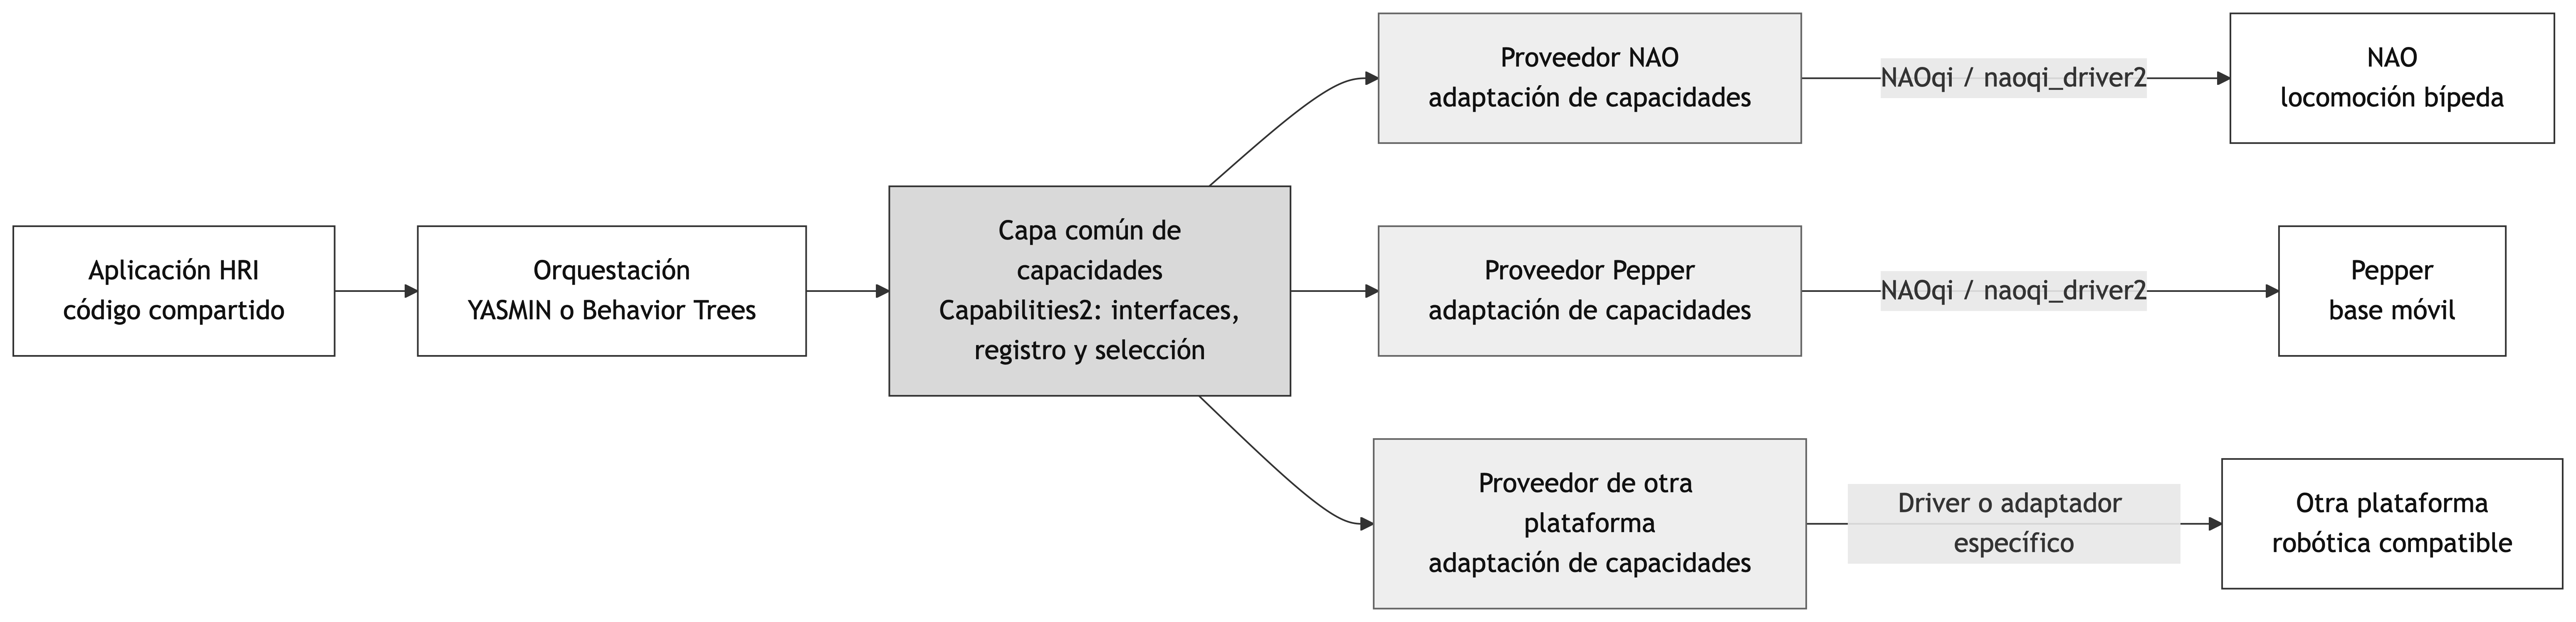
\includegraphics[width=\linewidth]{arquitectura_propuesta.png}
\caption{Separación entre aplicación, orquestación, capacidades y proveedores planteada en la propuesta original de agosto.}\label{fig:arquitectura}
\end{figure}

El diseño implementado emplea YASMIN para coordinar el comportamiento y Capabilities2 para adquirir, verificar y liberar proveedores. Los contratos públicos de ROS~2 transportan las detecciones, las órdenes de velocidad y los mensajes de voz. Este reparto permite cambiar el detector o el reconocedor, y concentrar la adaptación física en los recursos declarados en el perfil del robot.

\par\medskip\noindent\textbf{Reconocimientos y Agradecimientos}\par

El autor agradece a Mario Fernando De la Rosa Rosero por la dirección académica y técnica del proyecto, a David Cuevas Alba por la capacitación y el acompañamiento en el laboratorio, y al Departamento de Ingeniería de Sistemas y Computación y al grupo SinfonIA de la Universidad de los Andes por el acceso a los robots y a la infraestructura de integración.

\par\medskip\noindent\textbf{Diseño, implementación y resultados}\par

El sistema creció desde tres modos individuales hasta un comportamiento que escucha una orden, responde, detecta una persona y regula la marcha. Se verificó la interpretación de órdenes con audio sintético y se evaluó la regla de avance con detecciones previamente registradas. El ensayo físico reunió ambos cambios en NAO. La sección~\ref{sec:implementacion} presenta ambos mecanismos y la sección~\ref{sec:validacion} reconstruye los ensayos que motivaron el cambio. Pepper aportó evidencia de las funciones individuales en septiembre. Su indisponibilidad posterior impidió repetir en él la aplicación integrada. En el Hiwonder MentorPi se verificó la cadena de percepción con un perfil sin voz, sin llegar a mover la base.

\section{Descripción general}
\subsection{Objetivos}

El objetivo general y los siete objetivos específicos siguientes corresponden a la propuesta de agosto para trabajar con NAO y Pepper. La tabla~\ref{tab:objetivos} contrasta esas metas con el alcance de la evidencia al cierre.

\par\medskip\noindent\textbf{Objetivo General}\par

Diseñar, implementar y evaluar una arquitectura modular basada en capacidades sobre ROS~2 que favorezca la portabilidad y reutilización de aplicaciones de interacción humano-robot entre distintas plataformas robóticas mediante interfaces comunes y proveedores específicos, tomando a NAO y Pepper como plataformas iniciales de implementación y validación.

\par\medskip\noindent\textbf{Objetivos específicos}\par

\begin{enumerate}

\item Caracterizar las capacidades de interacción humano-robot requeridas y las diferencias funcionales y físicas entre plataformas, utilizando NAO y Pepper como casos iniciales para establecer cuáles pueden compartir una implementación y cuáles requieren proveedores específicos.

\item Diseñar una arquitectura modular sobre ROS~2 que separe las aplicaciones de alto nivel, la orquestación de comportamientos, los contratos comunes de capacidades, el registro y selección de proveedores y los adaptadores de hardware.

\item Implementar un prototipo de la arquitectura que permita registrar, seleccionar, ejecutar y sustituir proveedores, así como gestionar capacidades no disponibles, cancelaciones, errores y estados de ejecución.

\item Integrar proveedores iniciales para las capacidades de audio, percepción visual, navegación y detección de obstáculos, manipulación básica y generación de gestos, reutilizando componentes existentes y encapsulando las diferencias de las plataformas robóticas.

\item Implementar inicialmente la plataforma en NAO y Pepper mediante proveedores específicos para ambos robots y una aplicación HRI de referencia que combine varias capacidades y utilice únicamente las interfaces comunes de la arquitectura.

\item Evaluar la portabilidad y el funcionamiento de la solución mediante pruebas funcionales en las que se ejecute la misma aplicación de alto nivel en NAO y Pepper, reemplazando únicamente los proveedores específicos de cada plataforma.

\item Documentar la arquitectura, las interfaces, la configuración y el procedimiento para incorporar nuevos proveedores, capacidades o plataformas robóticas, con el propósito de facilitar su reutilización en proyectos futuros.

\end{enumerate}

\begin{table}[htbp]
\centering\small
\caption{Alcance alcanzado frente a los objetivos iniciales.}\label{tab:objetivos}
\begin{tabularx}{\linewidth}{@{}p{.7cm}P{3.3cm}Y@{}}
\toprule
N.º & Propósito & Evidencia al cierre \\
\midrule
1 & Caracterización & Inventario de sensores, servicios y candidatos de integración. Las pruebas de laboratorio verificaron una selección en NAO y Pepper. \\
2 & Separación modular & Seis contratos ROS~2, proveedores intercambiables, configuración de plataforma y aplicación Python/YASMIN. \\
3 & Gestión de proveedores & Adquisición, comprobación de identidad, vigilancia de comandos y liberación. Se documentaron fallos de disponibilidad y de cierre. \\
4 & Cobertura funcional & Voz, transcripción, personas en 2D, desplazamiento relativo y velocidad continua. Orientación de cámara con verificación parcial. Navegación autónoma, obstáculos, manipulación y gestos quedaron abiertos. \\
5 & Composición & Cuatro capacidades coordinadas físicamente en NAO. Tres funciones individuales confirmadas también en Pepper. \\
6 & Portabilidad & Reutilización física de las operaciones individuales en NAO y Pepper. La aplicación completa se evaluó en NAO. En el Hiwonder MentorPi se verificó la percepción sin actuación. El movimiento de esa plataforma sigue pendiente. \\
7 & Reproducción y extensión & Repositorios separados, perfil YAML, vocabulario configurable, versiones identificadas y registros de ensayo. La sección~\ref{sec:implementacion} incluye una guía de nodos, tópicos y servicios, y el apéndice~\ref{ap:repro} describe la reproducción. \\
\bottomrule
\end{tabularx}
\end{table}

\subsection{Antecedentes}
El desarrollo de software robótico reutilizable ha evolucionado desde arquitecturas estrechamente ligadas al hardware hacia enfoques basados en componentes, capacidades y habilidades (\emph{skills}). En estos enfoques la aplicación expresa qué debe hacer el robot, y módulos inferiores determinan cómo ejecutar la operación en una plataforma específica. ROS~2 proporciona la infraestructura de comunicación sobre la que se construyen estas propuestas, y su uso se ha documentado en robots desplegados en entornos terrestres, marítimos, aéreos y espaciales \cite{ros2}. Esta subsección revisa los trabajos que fundamentan la arquitectura, señala los contextos en que se han aplicado y precisa qué se adoptó de cada uno. Al final se describen las plataformas robóticas empleadas.

\par\medskip\noindent\textbf{Arquitecturas basadas en habilidades y capacidades}\par

Mayr, Rovida y Krueger presentan SkiROS2, una plataforma de control basada en habilidades que combina planificación automática, ejecución reactiva mediante árboles de comportamiento y un modelo semántico del mundo \cite{skiros}. Su formulación define, para cada habilidad, parámetros, precondiciones, condiciones que deben mantenerse durante la ejecución y postcondiciones. Los autores ilustran la plataforma con casos de uso que abarcan planificación de tareas, razonamiento, entradas multisensoriales, integración con un sistema de ejecución de manufactura y aprendizaje por refuerzo. El aporte más cercano a este proyecto es la separación entre la descripción de una habilidad y sus implementaciones: distintos dispositivos pueden implementar la misma descripción, y el sistema escoge la implementación compatible con el hardware. El artículo indica que la versión disponible se integraba con ROS~1 y que la adaptación a ROS~2 estaba en desarrollo. Por esta razón SkiROS2 se tomó como modelo conceptual. El prototipo conserva la idea de condiciones verificables: exige el acuse de una orden cero antes de habilitar el movimiento, vigila la continuidad del emisor y la antigüedad de los datos durante la ejecución y contrasta el desplazamiento relativo con la odometría al terminar.

Desde una perspectiva nativa de ROS~2, Pritchard y colaboradores presentan Capabilities2, una reimplementación del sistema \emph{Capabilities} para representar y ejecutar capacidades robóticas en aplicaciones de interacción humano-robot \cite{capabilities2}. El sistema distingue interfaces, proveedores e interfaces semánticas, y añade una arquitectura de complementos. Esta separación permite registrar una capacidad con independencia del nodo que la implementa y seleccionar el proveedor durante la ejecución. Capabilities2 no incluye capacidades de HRI ni adaptadores para robots concretos. Este proyecto adopta su servidor para registrar contratos, iniciar y liberar proveedores y vigilar el vínculo con el cliente \cite{capabilities2repo}, y aporta los contratos, los adaptadores y la aplicación de referencia. La separación permitió compartir un proveedor cuando dos robots exponen servicios compatibles, como ocurrió con la síntesis de voz en NAO y Pepper.

\par\medskip\noindent\textbf{Marcos de interacción humano-robot sobre ROS~2}\par

En relación directa con el hardware disponible, Bono y colaboradores proponen Open Access NAO (OAN), un marco ROS~2 para experimentación en HRI con NAO~V6 \cite{oan}. OAN instala en el robot un sistema operativo basado en Ubuntu y utiliza ROS~2 de forma nativa, sin las APIs de alto nivel del fabricante. Reúne caminata, reproducción y enseñanza de movimientos, captura de cámaras y audio, reconocimiento y síntesis de voz, detección de caras y objetos y conversación mediante modelos generativos, e incorpora simulación en Webots. OAN demuestra que las capacidades fundamentales de HRI pueden organizarse como módulos ROS~2 extensibles. Sin embargo, está diseñado únicamente para NAO~V6, requiere reemplazar el software de la plataforma y no aborda la interoperabilidad con otros robots. En este proyecto se mantuvo NAOqi y el controlador del laboratorio, y la portabilidad se buscó en una capa superior.

González-Santamarta y colaboradores presentan MERLIN2, una arquitectura cognitiva híbrida integrada con ROS~2 para generar, planificar, controlar y monitorizar comportamientos autónomos \cite{merlin2}. MERLIN2 distribuye el sistema en capas de misión, planificación, ejecución y reacción. En la capa reactiva ubica capacidades elementales, como navegación, reconocimiento de objetos, conversión de voz a texto y síntesis de voz, que las capas superiores combinan en acciones y planes. La implementación integra YASMIN, Nav2, herramientas PDDL y \code{yolo_ros}, y se evaluó en simulación y en un robot TIAGo real mediante una tarea de RoboCup@Home. El trabajo muestra que una base de capacidades puede sostener proyectos complejos de autonomía. Adoptar su infraestructura cognitiva completa excedía el alcance de este proyecto, que tomó de él la separación entre capacidades elementales y comportamiento.

Cooper y colaboradores introducen una arquitectura ROS~2 abierta y un simulador para robots sociales situados \cite{cooper}. El sistema combina percepción multimodal mediante ROS4HRI, una base de conocimiento, modelos de lenguaje y un controlador basado en intenciones que ejecuta tareas paralelas y secuenciales. Como complemento, el tutorial de Lemaignan y colaboradores muestra cómo ensamblar un robot social interactivo con ROS4HRI, ROS~2 y modelos de lenguaje \cite{ros4hritutorial}. ROS4HRI aplica las convenciones de REP-155 y ofrece una representación compartida de rostros, cuerpos, voces y personas, lo que evita que las aplicaciones dependan de un detector concreto \cite{ros4hri}. Estos trabajos orientaron la distinción entre detectar una persona, decidir seguirla y ejecutar una orden física. El prototipo implementa un mensaje propio de detecciones en 2D que incluye la marca de tiempo y la geometría necesarias para el control. La compatibilidad con ROS4HRI queda abierta.

\par\medskip\noindent\textbf{Orquestación, acceso al hardware y componentes reutilizables}\par

La coordinación de las capacidades requiere un mecanismo de ejecución. YASMIN permite definir comportamientos robóticos mediante máquinas de estados jerárquicas en ROS~2, con implementaciones en Python y C++, estados para acciones, servicios y tópicos y una memoria compartida entre estados \cite{yasmin,yasminrepo}. Su función en este proyecto es componer capacidades comunes en una aplicación, sin ocultar por sí mismo las diferencias de hardware.

En el nivel de acceso al hardware, \code{naoqi_driver2} ofrece el puente entre ROS~2 y NAOqi para NAO y Pepper \cite{naoqidriver}. El grupo SinfonIA de la Universidad de los Andes lo ha extendido mediante un metapaquete de arranque que agrupa el acceso a audio, cámaras, movimiento, voz y otras funciones \cite{sinfonia}. Estos desarrollos fueron el punto de partida local y actúan como controladores y envoltorios de las funciones del fabricante. Sus nombres de tópicos y servicios dependen del robot, por lo que una aplicación escrita directamente contra ellos hereda esa dependencia. En este proyecto se usaron sin modificaciones como capa de hardware.

Para las funciones de percepción y voz existen componentes abiertos que pueden actuar como proveedores. \code{yolo_ros} integra los modelos YOLO de Ultralytics en ROS~2 y ofrece detección, seguimiento y estimación de pose \cite{yoloros,ultralytics}. \code{whisper_ros} y \code{piper_ros} se consideraron en la propuesta para transcripción y síntesis de voz \cite{whisperros,piperros}. El prototipo utiliza \code{yolo_ros} con el modelo YOLOv8n para detectar personas, la síntesis de voz de NAOqi, el modelo Whisper \cite{whisper} para transcripción libre y el reconocedor Vosk \cite{vosk} para órdenes con vocabulario acotado. Cada uno queda encapsulado detrás de un contrato común, de modo que su sustitución no modifica la aplicación.

\par\medskip\noindent\textbf{Brecha identificada y posición del proyecto}\par

La revisión identifica una brecha concreta. SkiROS2 aporta el modelo de habilidades y la selección por hardware, pero no una base ROS~2 orientada a HRI. Capabilities2 ofrece mecanismos nativos de interfaces y proveedores, pero no capacidades para robots específicos. OAN integra funciones de HRI en NAO, pero no busca portabilidad hacia otras plataformas. MERLIN2 y el marco de Cooper y colaboradores muestran arquitecturas completas, validadas en otras plataformas o en simulación. En la revisión realizada para la propuesta no se identificó un trabajo que combinara una capa común de capacidades de HRI en ROS~2 con implementaciones para más de un robot y que evaluara de forma explícita la ejecución de una misma aplicación de alto nivel en ellos. Este proyecto se sitúa en esa brecha. La tabla~\ref{tab:antecedentes} resume la relación entre cada antecedente y el prototipo.

\begin{table}[htbp]
\centering\small
\caption{Antecedentes revisados y su relación con el prototipo.}\label{tab:antecedentes}
\begin{tabularx}{\linewidth}{@{}P{3.1cm}YY@{}}
\toprule
Antecedente & Aporte y contexto de aplicación & Relación con este proyecto \\
\midrule
SkiROS2 \cite{skiros} & Habilidades con precondiciones, condiciones de mantenimiento y postcondiciones. Casos de uso en planificación y manufactura. & Referencia conceptual. Comprobaciones antes, durante y después de ejecutar una capacidad. \\
Capabilities2 \cite{capabilities2} & Interfaces, proveedores y complementos en ROS~2 para HRI. & Adoptado como gestor de proveedores. \\
OAN \cite{oan} & Módulos de HRI nativos de ROS~2 para NAO~V6, con simulación. & Referencia funcional. Se conservó NAOqi y la portabilidad se resolvió en una capa superior. \\
MERLIN2 \cite{merlin2} & Arquitectura cognitiva por capas, evaluada en un TIAGo en una tarea de RoboCup@Home. & Referencia para separar capacidades y comportamiento. No se adoptó la planificación. \\
Cooper et al. y ROS4HRI \cite{cooper,ros4hritutorial} & Robots sociales situados y representación común de personas. & Mensaje propio de detecciones en 2D. Compatibilidad abierta. \\
YASMIN \cite{yasmin} & Máquinas de estados jerárquicas en ROS~2. & Adoptado para la orquestación. \\
\code{naoqi_driver2} y SinfonIA \cite{naoqidriver,sinfonia} & Acceso desde ROS~2 a NAO y Pepper. & Capa de hardware, sin modificaciones. \\
\code{yolo_ros}, Whisper y Vosk \cite{yoloros,whisper,vosk} & Detección de personas y reconocimiento de voz. & Encapsulados como proveedores intercambiables. \\
\bottomrule
\end{tabularx}
\end{table}

\par\medskip\noindent\textbf{Plataformas robóticas utilizadas}\par

El proyecto trabajó con tres plataformas de morfología distinta (tabla~\ref{tab:robots}). NAO es un humanoide bípedo de unos 0,57~m de altura, concebido como una plataforma abierta y asequible \cite{nao}. La unidad del laboratorio es un NAO~V6 con NAOqi~2.8. Pepper es un humanoide de aproximadamente 1,2~m, producido en serie y diseñado para la interacción con personas, que se desplaza sobre una base omnidireccional de tres ruedas y lleva una tableta en el pecho \cite{pepper}. Ambos comparten el sistema NAOqi y el controlador ROS~2 del laboratorio, y figuran entre los robots sociales que la literatura registra en servicios de atención al público \cite{socialrobots}. El Hiwonder MentorPi~M1 es un vehículo educativo basado en una Raspberry~Pi~5, con cuatro ruedas mecanum que le permiten desplazarse en cualquier dirección del plano, un lidar y una cámara de profundidad \cite{mentorpi}. No pertenece al ecosistema NAOqi y, en la configuración utilizada, no ofrece voz ni micrófono.

\begin{table}[htbp]
\centering\small
\caption{Plataformas robóticas del proyecto y recursos empleados en cada una.}\label{tab:robots}
\begin{tabularx}{\linewidth}{@{}P{2.5cm}YYY@{}}
\toprule
Aspecto & NAO & Pepper & Hiwonder MentorPi~M1 \\
\midrule
Morfología y locomoción & Humanoide bípedo. & Humanoide con base omnidireccional de ruedas. & Vehículo con cuatro ruedas mecanum. \\
Cámara utilizada & Frontal, $320\times240$ píxeles. & Cámara del controlador NAOqi. & De color, $640\times480$ píxeles. \\
Voz y audio & Síntesis de NAOqi y micrófonos. & Síntesis de NAOqi y micrófonos. & Sin voz ni micrófono en el perfil. \\
Acceso desde ROS~2 & Controlador SinfonIA/NAOqi, recursos bajo \code{/nao}. & Controlador SinfonIA/NAOqi, recursos bajo \code{/pepper}. & Software ROS~2 del fabricante, base en \code{/cmd_vel}. \\
Papel en el proyecto & Plataforma principal. Funciones individuales y aplicación integrada. & Segunda plataforma de las funciones individuales. Fuera de servicio desde noviembre. & Prueba de portabilidad hacia otro controlador y otra morfología. \\
\bottomrule
\end{tabularx}
\end{table}

\subsection{Identificación del problema y de su importancia}

El problema que aborda este proyecto es la dependencia de la lógica de interacción respecto de las APIs, los nombres de recursos y los comportamientos específicos de cada plataforma. Mientras esa dependencia exista, el conocimiento invertido en una aplicación queda ligado al robot para el que se escribió. Los antecedentes muestran que hay componentes de calidad para percibir, hablar y moverse. Lo que falta es una forma común de componerlos que sobreviva al cambio de robot.

\par\medskip\noindent\textbf{Un campo en expansión}\par

La relevancia del problema crece con la adopción de los robots sociales. Vishwakarma y colaboradores \cite{socialrobots} combinan un análisis bibliométrico, realizado con metadatos de Scopus, y una revisión sistemática de 79 artículos publicados entre 2012 y febrero de 2023, seleccionados de Scopus, Web of Science, EBSCO Business Source Complete y Google Scholar. Los autores describen un campo reciente y en crecimiento. La producción de artículos sobre adopción comienza en 2016, y más de la mitad de los estudios revisados se publicó en 2020 y 2021. La revisión recoge además que los robots sociales ocuparon el segundo lugar entre las diez tecnologías emergentes de 2019 según el Foro Económico Mundial y \emph{Scientific American}, y que para su mercado se proyecta una tasa de crecimiento anual compuesta del 32,4~\% hasta 2028.

Los robots sociales se han adoptado principalmente en las industrias de viajes, turismo, hotelería y hospitalidad, a las que corresponde el 39,24~\% de los estudios revisados. Siguen la banca y las finanzas, la salud, la moda, el comercio minorista y el sector legal. Los dos humanoides de este proyecto figuran entre los ejemplos de la revisión. Esta menciona a Pepper en la recepción de un hotel y en funciones de atención al cliente en aeropuertos, restaurantes y comercios, y a NAO en servicios de primera línea en hoteles y en la atención de sucursales bancarias. Los autores señalan que la pandemia de COVID-19 aceleró el uso de estos robots en servicios de recepción, y que la demanda en el sector de servicios va en aumento aunque la adopción se encuentra todavía en una etapa inicial.

\par\medskip\noindent\textbf{Desafíos de la adopción y dimensión tecnológica}\par

La misma revisión muestra que la adopción no está asegurada. Clasifica sus desafíos en psicológicos, éticos, sociales, operativos, técnicos, financieros, organizacionales, de recursos humanos y regulatorios. Entre ellos figuran la complejidad de la tecnología, la calidad deficiente de los algoritmos entregados por los proveedores, la falta de soporte de infraestructura, la alta inversión inicial y la ausencia de estándares de industria definidos por las autoridades. Señala también que el mantenimiento y la reparación de los robots y de sus sensores, sistemas y algoritmos exigen inversiones posteriores, y que muchas organizaciones carecen de conocimiento suficiente sobre inteligencia artificial y robótica. Como ilustración, documenta el caso de un hotel en Japón que retiró la mitad de sus robots de atención al cliente porque fallaban con frecuencia y su reparación elevaba los costos.

Para explicar la adopción, los autores proponen un marco de investigación que extiende el esquema de antecedentes, decisiones y resultados con el marco tecnológico-organizacional-ambiental. En él, los antecedentes tecnológicos son una infraestructura de tecnologías de información adecuada, la capacidad de innovación tecnológica y la disponibilidad de personal experto, y el soporte de hardware y software se identifica como un factor crítico de éxito.

De ese panorama se derivan tres implicaciones para este trabajo. La primera es que los robots sociales ya operan fuera del laboratorio, en servicios donde atienden a personas. Las aplicaciones que los gobiernan deben entonces mantenerse, corregirse y trasladarse a lo largo de su vida útil, y no solo demostrarse una vez. La segunda es que varios de los desafíos documentados son de naturaleza técnica y se agravan cuando la aplicación está acoplada al robot. Si cada plataforma nueva obliga a reescribir la lógica de interacción, la complejidad y la dependencia de personal experto se repiten con cada adquisición. La tercera es que un componente puede resultar inadecuado para las condiciones reales de uso y que los robots fallan. Una arquitectura con contratos comunes actúa sobre esos puntos: reduce lo que debe reescribirse, permite sustituir un componente sin modificar la aplicación y deja continuar el trabajo en otra plataforma cuando una queda fuera de servicio. Ambas situaciones se presentaron en este proyecto, con el cambio del reconocedor de voz y con la indisponibilidad de Pepper.

La revisión estudia la adopción desde la gestión de las operaciones de servicio y no evalúa arquitecturas de software. La relación entre sus hallazgos y la portabilidad es un argumento de este trabajo, que no midió costos ni tasas de adopción.

\par\medskip\noindent\textbf{Heterogeneidad de las plataformas}\par

Las organizaciones y los laboratorios rara vez disponen de un único modelo de robot. En este proyecto coincidieron un humanoide bípedo, un humanoide con base de ruedas y un vehículo con ruedas mecanum. Sus cámaras entregan imágenes de distinto tamaño, sus controladores usan nombres de recursos diferentes y solo dos de ellos pueden hablar y escuchar. Una aplicación escrita contra los recursos de uno de ellos tendría que modificarse para cada uno de los demás. Con contratos comunes, esas diferencias se declaran en un perfil y se resuelven en los proveedores.

La disponibilidad de los robots también cambia. Durante el proyecto, Pepper quedó fuera de servicio tras un accidente. El trabajo continuó en NAO con la misma aplicación porque esta no dependía de recursos propios de Pepper. Este episodio ilustra un riesgo concreto del acoplamiento: cuando la lógica de interacción está atada a una plataforma, la falla de esa plataforma detiene también el desarrollo de la aplicación.

\par\medskip\noindent\textbf{Localización de fallos}\par

La dependencia directa dificulta además distinguir errores de interacción, de integración y de hardware. Durante el desarrollo aparecieron fallos de los tres tipos: una regla de avance inadecuada para una cámara baja, una comprobación de identidad que dependía de la implementación de DDS y sesiones de NAOqi desconectadas. La separación en capas permitió atribuir cada uno a la aplicación, al proveedor o al controlador, y corregirlo en un solo lugar. La sección~\ref{sec:validacion} documenta estos casos.

\par\medskip\noindent\textbf{Alcance de la afirmación}\par

La importancia práctica del trabajo radica en reducir la duplicación y en facilitar nuevos experimentos sobre la infraestructura existente. Los beneficios económicos o de productividad son expectativas, no resultados medidos en este proyecto. La portabilidad tampoco elimina las responsabilidades de seguridad: una instrucción equivalente puede producir movimientos diferentes según el robot, su entorno y el estado de sus controladores. Por ello cada plataforma requiere su propia verificación física, aunque la aplicación sea la misma.

\section{Diseño y especificaciones}
\subsection{Definición del problema}
Dada una persona frente al robot, la aplicación debe permanecer en pausa hasta reconocer una orden de seguir, girar y avanzar con información visual reciente y volver a la pausa ante una orden de detención. La escena prevista contiene una sola persona elegible. La aplicación recibe cajas de detección en la imagen y sus marcas de tiempo. El perfil define la cámara y los límites aceptables de movimiento. La estimación de cercanía es visual y depende del campo de visión.

\subsection{Especificaciones}
\par\medskip\noindent\textbf{Requerimientos funcionales}\par
\begin{enumerate}[label=RF\arabic*.]
\item Registrar, adquirir y liberar proveedores. Antes de habilitar movimiento, comprobar que el proveedor seleccionado responde a una orden cero de la aplicación.
\item Exponer las funciones individuales de síntesis de voz, detección de personas y desplazamiento relativo. En este último, contrastar el objetivo con la odometría del robot.
\item Distinguir un cuadro reciente sin personas, varias personas, ausencia de datos y geometría inválida. Para iniciar o reanudar el seguimiento exigir tres observaciones nuevas y válidas de una sola persona elegible.
\item Convertir la posición y el tamaño aparentes de la persona en consignas acotadas de avance y giro. Conservar la base detenida mientras no haya información suficiente.
\item Reconocer en español órdenes completas dirigidas al robot, responder en voz alta y mantener la pausa solicitada hasta recibir una nueva orden de seguir.
\item Centralizar en el perfil los proveedores, modelos, recursos ROS y umbrales visuales de la plataforma. Registrar decisiones, esperas, estados de voz y datos de rendimiento para reconstruir una sesión.
\end{enumerate}

\par\medskip\noindent\textbf{Requerimientos no funcionales y criterios de aceptación}\par
Los recursos específicos del robot deben poder cambiarse desde el perfil. Cada prueba debe identificar el proveedor y permitir reconstruir por qué el controlador avanzó o retuvo la base. En la configuración final, una detección con antigüedad superior a 0,75~s impide el avance. La evaluación del movimiento utiliza velocidades comandadas y observación del operador cuando no hay una medición externa.

Para los modos individuales se exige el efecto correspondiente: voz audible, detección de personas en la imagen o desplazamiento relativo observado y contrastado con odometría. Los umbrales del modo de desplazamiento fueron 0,05~m de diferencia planar y 0,15~rad de diferencia angular. Para el ensayo integrado el criterio fue completar, dentro de la misma sesión física, pausa inicial, orden de seguir, seguimiento observado, orden de detenerse y vuelta a pausa. Para afirmar portabilidad del comportamiento completo se necesita repetir esa secuencia en una segunda plataforma con la misma lógica de alto nivel.

\subsection{Restricciones}
La cámara frontal de NAO entrega una vista monocular desde una posición baja. Una caja puede ocupar casi toda la altura de la imagen aun cuando la persona esté a cierta distancia. La red, la cámara del robot y la capacidad de cómputo del equipo del laboratorio afectan la antigüedad de las detecciones. Por ello, las métricas de la sesión se informan con su ventana de observación.

Cada prueba física se realizó bajo supervisión. La orden verbal de pausa forma parte de la interacción. La confirmación de un comando cero por el proveedor informa del estado de la cadena de mando. La distancia y el tiempo mecánico de frenado requerirían instrumentos externos. La aplicación no planifica rutas ni evita obstáculos. El despliegue evaluado presupone una única aplicación con control del movimiento y utiliza los nombres comunes de recursos dentro de un dominio ROS.

El proyecto empleó el hardware del laboratorio y software existente, sin financiación específica. La evaluación técnica no requirió conformar una base de datos de participantes. La cámara y el micrófono se procesaron durante la ejecución. El observador de la sesión final registró estados, tiempos y métricas técnicas.

\section{Desarrollo del diseño}
Se avanzó del control individual de las capacidades a una tarea que obligaba a coordinarlas. El desplazamiento relativo permitió comprobar odometría y tolerancias con un objetivo fijo. Para seguir a una persona en movimiento fue necesario enviar consignas sucesivas y dejar de aplicarlas si la fuente de datos o el emisor de órdenes se perdían. El control continuo exigió, por tanto, un contrato diferente y una comprobación explícita de parada.

\subsection{Recolección de información}
La caracterización inicial reunió documentación de NAOqi y SinfonIA, interfaces disponibles en ROS~2 y antecedentes académicos. En el laboratorio se contrastó ese inventario con servicios de voz y movimiento y tópicos de batería, sonar, cámara, micrófono y odometría. La disponibilidad de un tópico permitió identificar una entrada candidata. Para evaluar una función se exigió además una prueba que la utilizara.

En las etapas de integración se asociaron la marca de tiempo de la imagen, el instante de recepción y la decisión del controlador. Durante las comparaciones de noviembre se añadió un observador independiente de percepción, voz y carga del sistema. Así pudo distinguirse una pausa causada por datos visuales antiguos de otra debida a indisponibilidad del micrófono.

\subsection{Alternativas de diseño}
\begin{table}[htbp]
\centering\small
\caption{Decisiones de diseño y consecuencias observables.}
\begin{tabularx}{\linewidth}{@{}P{3.8cm}YY@{}}
\toprule
Decisión & Alternativa & Consecuencia en el prototipo \\
\midrule
Contratos y perfil por robot & Llamadas directas al controlador & El comportamiento usa nombres comunes. El perfil y los proveedores resuelven los recursos específicos. \\
YASMIN en Python & Árbol de comportamiento & Los estados hacen explícita la prioridad de la pausa y dejan rastros de adquisición, seguimiento y liberación. \\
Flujo de detecciones & Consulta puntual & Cada mensaje indica qué imagen originó la detección. Un cuadro vacío se distingue de una interrupción. \\
Velocidad continua & Encadenar desplazamientos relativos & Se puede corregir la dirección ante cada observación y enviar cero mientras se exige información reciente. \\
Vosk con vocabulario acotado & Whisper para transcripción libre & La política acepta una instrucción completa y mantiene la pausa al fallar la escucha. Los ensayos de CPU y audio se presentan en la sección~\ref{sec:validacion}. \\
Ancho relativo de la caja & Altura relativa & En una cámara baja, el ancho puede seguir siendo válido cuando la cabeza o los pies quedan fuera del encuadre. \\
\bottomrule
\end{tabularx}
\end{table}

\FloatBarrier
\section{Implementación}\label{sec:implementacion}
\subsection{Descripción de la implementación}

\par\medskip\noindent\textbf{Entorno y organización}\par

El desarrollo inicial utilizó Docker con ROS~2 Jazzy para construir y probar componentes en el computador del autor. Las pruebas físicas se ejecutaron en el laboratorio con Ubuntu 24.04, arquitectura x86\_64 y ROS~2 Jazzy. El driver SinfonIA/NAOqi se mantiene en un workspace separado y el software propio se construye como overlay.

Los repositorios del proyecto separan documentación, contratos, proveedores y sistema de referencia: \code{portable-hri-docs} \cite{repodocs}, \code{portable-hri-interfaces} \cite{repointerfaces}, \code{portable-hri-providers} \cite{repoproviders} y \code{portable-hri-reference-system} \cite{reposystem}. Esta distribución permite distinguir la interfaz reutilizable, su implementación y las aplicaciones y pruebas que la consumen. Los repositorios contienen el detalle de cada mensaje, parámetro y prueba. Este informe presenta una guía resumida.

La figura~\ref{fig:actual} muestra qué selecciona el perfil y dónde termina la responsabilidad de la aplicación. Los mensajes funcionales circulan entre los nodos ROS~2. El servidor Capabilities2 administra la adquisición y liberación del proveedor, comprueba el vínculo con el cliente y permite verificar qué implementación está activa. Las imágenes y el audio llegan a los procesos de percepción y voz a través de suscripciones.

\begin{figure}[!htb]
\centering
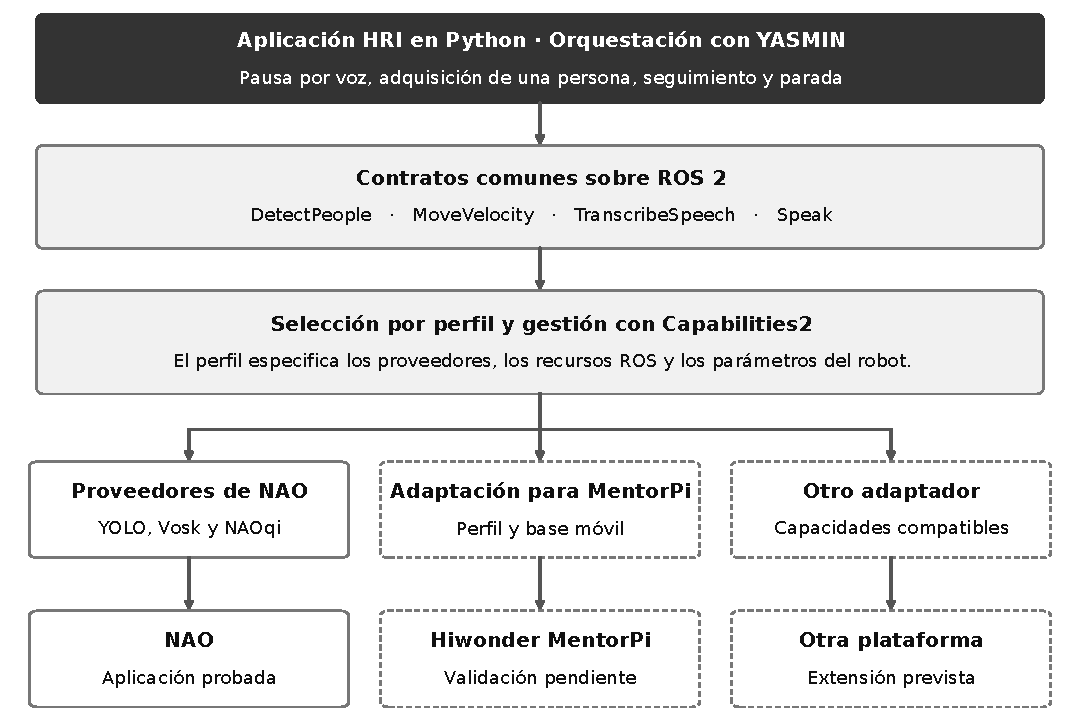
\includegraphics[width=.90\linewidth]{arquitectura_implementada.pdf}
\caption{Arquitectura de la aplicación integrada. Los recuadros con borde discontinuo indican adaptaciones previstas o sin verificación física completa. La rama NAO corresponde al ensayo físico completo.}\label{fig:actual}
\end{figure}

\par\medskip\noindent\textbf{Contratos y proveedores}\par
La tabla~\ref{tab:catalogo} presenta las seis capacidades definidas, el intercambio que establece cada contrato y el proveedor que lo implementa.
\begin{table}[htbp]
\centering\small
\caption{Catálogo de capacidades y uso durante las pruebas.}\label{tab:catalogo}
\begin{tabularx}{\linewidth}{@{}P{3.15cm}YY@{}}
\toprule
Capacidad & Intercambio funcional & Implementación y uso \\
\midrule
\code{Speak} & Texto e idioma en \code{/hri/speak}, con confirmación o error. & \code{NaoSpeak} adapta el servicio de voz de NAOqi. Se reutilizó en Pepper mediante remapeo. En la sesión integrada respondió a las órdenes. \\
\code{DetectPeople} & Flujo \code{/hri/people} con marca de tiempo y cajas 2D. Un cuadro sin personas contiene una lista vacía. & \code{YoloDetectPeople} adapta las detecciones de YOLO. La aplicación consulta la calidad y la antigüedad de cada observación. \\
\code{MoveRelative} & Objetivo planar $(x;\,y;\,\theta)$ relativo al marco inicial y estimación por odometría. & El proveedor NAOqi combina \code{move_to} y \code{odom}. Se probó como modo individual en ambos humanoides. \\
\code{MoveVelocity} & Consignas \code{Twist} en \code{/hri/cmd_vel} y estado en \code{/hri/move_velocity/status}. & El proveedor NAOqi vigila la continuidad del emisor y de la orden. El seguimiento lo usa para avanzar, girar y pedir parada. \\
\code{TranscribeSpeech} & Audio procesado por el proveedor, estado de captura y texto reconocido para la aplicación. & Se implementaron proveedores para Whisper y Vosk. Vosk reconoció el vocabulario de órdenes de la prueba final. \\
\code{OrientCamera} & Solicitud de orientación e información de estado. & Proveedor opcional para el movimiento de cabeza. Verificado con interfaces simuladas y desactivado en el ensayo final. \\
\bottomrule
\end{tabularx}
\end{table}

\par\medskip\noindent\textbf{Guía de nodos, tópicos y servicios}\par
Esta guía resume los elementos de ROS~2 que intervienen en la aplicación integrada. Se organiza en tres niveles: los procesos que se ejecutan (tabla~\ref{tab:nodos}), los recursos públicos que la aplicación conoce (tabla~\ref{tab:recursos}) y los recursos propios de cada robot, que solo aparecen en el perfil y en los proveedores (tabla~\ref{tab:backend}). Las definiciones completas se encuentran en los repositorios de interfaces, proveedores y sistema de referencia \cite{repointerfaces,repoproviders,reposystem}.

\begin{table}[htbp]
\centering\small
\caption{Procesos de la aplicación integrada y función de cada uno.}\label{tab:nodos}
\begin{tabularx}{\linewidth}{@{}P{3.6cm}P{3.3cm}Y@{}}
\toprule
Proceso o nodo & Paquete & Función \\
\midrule
\code{hri_app} & \code{hri_reference_app} & Aplicación. Ejecuta la máquina de estados YASMIN, adquiere las capacidades, aplica la regla de seguimiento y la política de órdenes de voz y publica las consignas de velocidad. \\
\code{capabilities2_server_node} & \code{capabilities2} & Servidor de capacidades. Registra contratos y proveedores, inicia y libera el ejecutor de cada proveedor y vigila el vínculo con la aplicación. \\
Ejecutores de proveedores & \code{hri_naoqi_providers}, \code{hri_yolo_providers}, \code{hri_vosk_providers}, \code{hri_whisper_providers} & Complementos que el servidor carga al adquirir una capacidad: \code{NaoSpeak}, \code{NaoqiMoveRelative}, \code{NaoqiMoveVelocity}, \code{NaoqiOrientCamera}, \code{YoloDetectPeople}, \code{VoskTranscribeSpeech} y \code{WhisperTranscribeSpeech}. Traducen el contrato común a los recursos del robot. \\
\code{yolo_node} & \code{yolo_ros} & Detector. Procesa la imagen de la cámara indicada en el perfil y publica las detecciones que consume \code{YoloDetectPeople}. \\
\code{vosk_worker} o \code{whisper_worker} & \code{hri_vosk_providers}, \code{hri_whisper_providers} & Reconocedor de voz. Procesa el audio del micrófono del robot para el proveedor de transcripción seleccionado. \\
\code{hri_diagnostics} & \code{hri_reference_app} & Observador opcional. Registra frecuencias, antigüedad de los datos, tiempos por estado y carga del sistema en \code{summary.json} y \code{events.jsonl}. \\
Controlador del robot & Externo al proyecto & Expone cámara, micrófono, odometría y servicios de voz y movimiento. Se inicia por separado. \\
\bottomrule
\end{tabularx}
\end{table}

\begin{table}[htbp]
\centering\small
\caption{Recursos públicos de los contratos. Los tipos propios pertenecen al paquete \texttt{hri\_capability\_interfaces}.}\label{tab:recursos}
\begin{tabularx}{\linewidth}{@{}P{4.3cm}P{1.5cm}P{4.2cm}Y@{}}
\toprule
Recurso & Clase & Tipo & Contenido \\
\midrule
\code{/hri/speak} & Servicio & \code{srv/Speak} & Texto e idioma. Responde éxito, proveedor y mensaje. \\
\code{/hri/people} & Tópico & \code{msg/PersonDetection2DArray} & Marca de tiempo de la imagen y, por persona, confianza, centro, ancho y alto de la caja. \\
\code{/hri/detect_people} & Servicio & \code{srv/DetectPeople} & Consulta puntual con confianza mínima y antigüedad máxima. \\
\code{/hri/move_relative} & Servicio & \code{srv/MoveRelative} & Objetivo $(x;\,y;\,\theta)$. Responde el desplazamiento alcanzado según la odometría. \\
\code{/hri/cmd_vel} & Tópico & \code{geometry_msgs/msg/Twist} & Consigna continua de avance y giro. \\
\code{/hri/move_velocity/status} & Tópico & \code{std_msgs/msg/String} & Estado del proveedor de velocidad y acuse de parada. \\
\code{/hri/speech/transcribe} & Servicio & \code{srv/TranscribeSpeech} & Inicio de una captura puntual o continua. \\
\code{/hri/speech/transcript} & Tópico & \code{msg/SpeechTranscript} & Texto reconocido, idioma e indicador de resultado final. \\
\code{/hri/speech/capture_status} & Tópico & \code{msg/SpeechCaptureStatus} & Estado de la captura y fragmentos en cola o descartados. \\
\code{/hri/camera/orient} & Servicio & \code{srv/OrientCamera} & Elevación solicitada para la cámara. \\
\code{/hri/camera/orientation} & Tópico & \code{msg/CameraOrientation} & Orientación medida y estado del movimiento. \\
\code{/capabilities/use_capability}, \code{/capabilities/free_capability} y \code{/capabilities/establish_bond} & Servicios & Capabilities2 & Adquisición y liberación de una capacidad y vínculo entre la aplicación y el servidor. \\
\bottomrule
\end{tabularx}
\end{table}

\begin{table}[htbp]
\centering\small
\caption{Recursos propios de cada plataforma. La aplicación no los nombra: el perfil y los proveedores los resuelven.}\label{tab:backend}
\begin{tabularx}{\linewidth}{@{}P{2.6cm}YYY@{}}
\toprule
Función & NAO & Pepper & Hiwonder MentorPi \\
\midrule
Imagen para el detector & \code{/nao/camera/front/image_raw} & Cámara del controlador, bajo \code{/pepper}. & \code{/ascamera/camera_publisher/rgb0/image} \\
Audio & \code{/nao/mic_stamped} y \code{/nao/mic_info} & \code{/pepper/mic_stamped} y \code{/pepper/mic_info} & No declarado. \\
Síntesis de voz & Servicio \code{/nao/say} & Servicio \code{/pepper/say} & No declarada. \\
Desplazamiento relativo & \code{/nao/move_to} y \code{/nao/odom} & \code{/pepper/move_to} y \code{/pepper/odom} & No utilizado. \\
Velocidad continua & \code{/nao/cmd_vel} & \code{/pepper/cmd_vel} & \code{/cmd_vel} \\
\bottomrule
\end{tabularx}
\end{table}

El recorrido de un dato ilustra la relación entre los tres niveles. El controlador publica la imagen de la cámara. \code{yolo_node} la procesa y publica detecciones en \code{/yolo/detections}. El proveedor \code{YoloDetectPeople} filtra las personas, conserva la marca de tiempo de la imagen y publica en \code{/hri/people}. La aplicación lee ese tópico, decide una consigna y la publica en \code{/hri/cmd_vel}. El proveedor de velocidad la limita, la vigila y la reenvía al tópico de la base del robot. En Pepper, los recursos de audio y de velocidad continua de la tabla~\ref{tab:backend} se inventariaron en septiembre, pero la aplicación no llegó a utilizarlos.

La máquina de estados de \code{follow_person} sigue un orden fijo. Primero establece el vínculo con el servidor y, si el perfil declara voz, emite el saludo. Luego adquiere \code{DetectPeople}, verifica el proveedor y configura la escucha. Si el movimiento está habilitado, adquiere \code{MoveVelocity} y espera el acuse de una orden cero. Después permanece en el estado de seguimiento hasta que el operador termina la sesión o se produce un fallo. Al salir, solicita la parada y libera las capacidades adquiridas. Además de los recursos de la tabla~\ref{tab:recursos}, la aplicación publica en \code{/hri/follow_person/preview} la decisión tomada ante cada imagen, que es la fuente del observador de diagnóstico.

Para incorporar otro robot se escribe un perfil en \code{hri_reference_app/config} con la geometría de su cámara, los proveedores elegidos y los recursos de la tabla~\ref{tab:backend}. Solo se requiere un proveedor nuevo cuando ninguno de los existentes puede traducir el contrato a la interfaz del robot.

\par\medskip\noindent\textbf{Dos recorridos de movimiento}\par
El modo individual \code{move_relative} recibe una posición y un ángulo. Dado que el servicio \code{MoveTo} del driver devuelve una respuesta vacía, el proveedor compara el estado inicial y final por odometría antes de informar el cumplimiento. El modo \code{follow_person} necesita reaccionar a cada detección, por lo que usa la capacidad independiente \code{MoveVelocity}. Al activar el control continuo, la aplicación envía ceros y espera un acuse nuevo. El proveedor limita las órdenes y exige una fuente válida de comandos. Ante pérdida de autorización o conflicto de emisores, la aplicación solicita una parada y libera sus recursos.

\par\medskip\noindent\textbf{Regla de seguimiento visual}\par
Sea $W$ el ancho de la imagen, $w$ el ancho de la caja de la persona y $u$ su coordenada horizontal central en píxeles. La cercanía aparente se expresa mediante $r=w/W$, y el error horizontal normalizado mediante $e=(u-W/2)/(W/2)$. El primero regula el avance y el segundo el giro. El controlador acepta como candidatas las detecciones de personas de YOLO con una puntuación de confianza de al menos 0,65. El valor de referencia $r=0{,}33$ indica la fracción del ancho que ocupa una caja, aproximadamente 106 píxeles en una imagen de 320. Cada parámetro responde por tanto a una pregunta diferente.

Con el perfil de NAO se propone avance para $r<0{,}30$. Entre $0{,}30$ y $0{,}36$ se retiene el avance y se permite corregir el giro. Por encima de esa banda también se retiene el avance. Cuando la persona está centrada, la consigna alcanza un máximo de 0,10~m/s para $r\leq 0{,}18$. El controlador reduce esa consigna hasta un tercio a medida que el centro de la persona se aparta entre 24 y 60~px del centro de la imagen de 320~px. El giro se limita a $0{,}10$~rad/s en magnitud. La figura~\ref{fig:control} separa los dos efectos para mostrar por qué NAO puede corregir el rumbo mientras avanza despacio.

\begin{figure}[htbp]
\centering
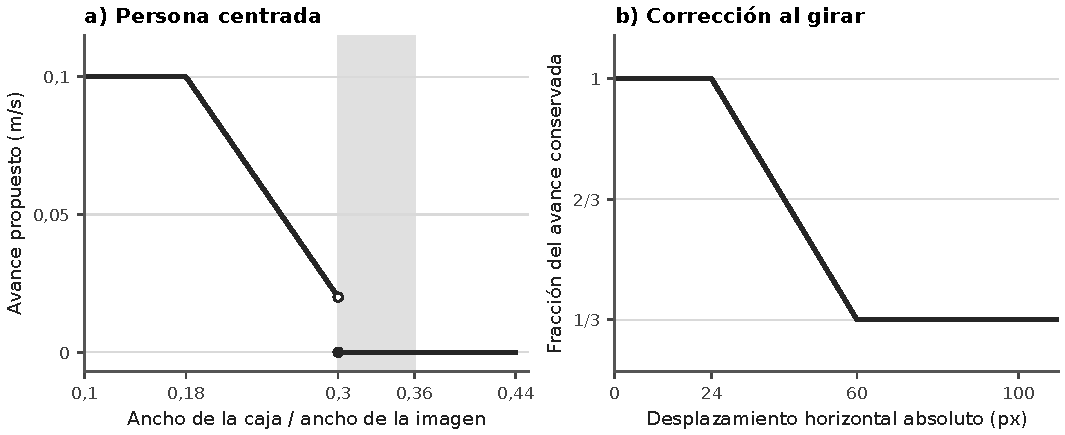
\includegraphics[width=\linewidth]{regla_seguimiento_nao.pdf}
\caption{Consigna de avance del perfil NAO para una detección elegible. En (a) la franja gris es la banda de cercanía. En (b) se muestra el factor que multiplica el avance de (a). Las curvas representan decisiones del controlador.}\label{fig:control}
\end{figure}

Se necesitan tres observaciones nuevas para adquirir o recuperar un objetivo. En modo de ancho, una caja que toca el borde superior o inferior conserva información horizontal utilizable. Si toca un borde lateral, el controlador pide cero en ambos ejes. Mientras falten imágenes recientes o haya cero o varias personas, la versión de noviembre conserva la sesión en espera y solicita velocidad cero. La reaparición de una persona permite reanudar un seguimiento autorizado. Una pausa solicitada por voz requiere además una nueva orden verbal. Esta regla reconoce una única detección elegible en el encuadre y no determina la identidad de quien vuelve a aparecer.

\par\medskip\noindent\textbf{Interacción por voz y ejecución integrada}\par
La entrada \code{aplicacion_hri.launch.py} inicia la aplicación, Capabilities2, YOLO y el proceso de reconocimiento indicado en el perfil. El driver físico se inicia aparte. Por defecto, la versión del 17 de noviembre usa Vosk con un modelo pequeño en español y arranca en pausa. Una transcripción final debe coincidir con la palabra de activación y con una frase de la lista configurada, como «NAO, sígueme» o «NAO, detente». La política ignora resultados parciales, repetidos o fuera de esa lista. La síntesis de voz se hace a través de \code{Speak} y se inhibe el reconocimiento de la respuesta del propio robot durante la locución y un segundo adicional.

Whisper permanece disponible para transcripción libre. Cambiar el motor de voz no cambia el contrato que consume el seguimiento. En la composición por órdenes, si se pierde el flujo de audio, el robot mantiene la pausa. La pérdida de audio por tiempo agotado en la versión evaluada requirió relanzar la aplicación para recuperar la escucha. En cambio, una interrupción visual recuperable puede resolverse en la misma sesión.

\subsection{Resultados esperados}
Se definieron dos criterios para evaluar la implementación. El primero fue que una persona pudiera iniciar y detener el seguimiento de NAO con la voz en una sola sesión. El segundo fue conservar la lógica de interacción al cambiar de plataforma. Para el primero se registraron transiciones, consignas y observación física. Para el segundo se examinó el código común usado en NAO y Pepper y se preparó un perfil para el Hiwonder MentorPi. La sección siguiente separa las ejecuciones efectivamente observadas de las adaptaciones que quedaron sin verificar.

\FloatBarrier
\section{Validación}\label{sec:validacion}
\subsection{Métodos}
\begin{enumerate}
\item \textbf{Pruebas con interfaces simuladas.} Nodos, servicios, receptores de velocidad, detecciones y audio de prueba permitieron controlar los estímulos, reproducir fallos y verificar selección, consignas, recuperación y liberación. También se reevaluaron cajas previamente registradas, sin activar los actuadores.
\item \textbf{Pruebas físicas con registros.} Se contrastó la ejecución en el laboratorio con observación del operador, salidas estructuradas, odometría en los recorridos relativos y tiempos del observador en la aplicación integrada. En los casos en que se conservó únicamente una confirmación cualitativa se informa expresamente.
\end{enumerate}

En movimiento, se comparan objetivo y desplazamiento estimado en el marco inicial. Para las tablas se usa la diferencia planar
\begin{equation}
e_p = \sqrt{(x_{\mathrm{estimado}}-x_{\mathrm{solicitado}})^2+(y_{\mathrm{estimado}}-y_{\mathrm{solicitado}})^2},
\end{equation}
y la magnitud de la diferencia angular normalizada. Esta comparación mide consistencia con la odometría, no error respecto de una referencia física externa.

\subsection{Validación de resultados}
La tabla~\ref{tab:semanas} organiza las semanas con evidencia disponible. Para las etapas posteriores a las bitácoras numeradas se indica la fecha real. La existencia de una actividad en el cronograma de la propuesta no se trató como registro de una ejecución.

\begin{table}[htbp]
\centering\small
\caption{Cronología del desarrollo y criterio observado en cada etapa de 2026.}\label{tab:semanas}
\begin{tabularx}{\linewidth}{@{}P{3.45cm}Y@{}}
\toprule
Semana o fecha & Actividad y evidencia \\
\midrule
19 de agosto & Propuesta de arquitectura y plan de trabajo. Punto de partida documental. \\
Semana 6, 9 de septiembre & Caracterización de capacidades y servicios. Comunicación ROS~2 en Docker y evaluación del servidor Capabilities2 con proveedores de prueba. \\
Semana 7, 16--17 de septiembre & Conexión desde el laboratorio. Comprobación de sensores y pronunciación audible en NAO y Pepper. \\
Semana 8, 22--23 de septiembre & Detección continua de personas, movimiento relativo con odometría y ejecución de los tres modos individuales de la aplicación. \\
27 de septiembre & Consolidación de las pruebas iniciales en el informe de avance. \\
14 de octubre & Implementación y prueba de velocidad continua. Dos consignas de avance y parada observada en NAO. \\
Semana 11, 19 y 21 de octubre & Seguimiento con y sin actuación, velocidad configurable, corrección de la identidad del emisor y evaluación de cámara y transcripción opcionales. \\
25 de octubre & Protocolo de gestión de datos y almacenamiento del proyecto. Hito documental. \\
4 de noviembre & Recuperación ante interrupciones de imagen y detecciones ambiguas. Ensayos físicos comparativos con Whisper y sin escucha. \\
11 de noviembre & Pruebas de órdenes con Vosk, diagnóstico de interrupciones de audio y cámara, y comparación de la política de recepción de imágenes. \\
17 de noviembre & Revisión de la regla de avance y prueba física completa en NAO, desde «sígueme» hasta «detente». \\
\bottomrule
\end{tabularx}
\end{table}
\FloatBarrier

\par\medskip\noindent\textbf{Septiembre. Pruebas de software}\par

\begin{table}[htbp]
\centering\small
\caption{Pruebas de software de los primeros incrementos, hasta el 23 de septiembre.}\label{tab:software}
\begin{tabularx}{\textwidth}{P{4cm}P{2.2cm}Y}
\toprule
Prueba & Resultado & Interpretación \\
\midrule
Comunicación ROS~2 en Docker & 7 coincidentes de 8 publicados & Comunicación C++ a Python dentro del contenedor; no demuestra descubrimiento en la red del laboratorio. \\
Núcleo Capabilities2 & 12/13 & Prueba global fallida: código de éxito incorrecto para proveedor inexistente. \\
Proveedor de voz & 9/9 por configuración & Destinos NAO y Pepper simulados; no equivalen a audio físico. \\
Personas, versión de consulta & 12/12 & Prueba de la primera versión del contrato. \\
Personas, flujo continuo & 14/14 & Incluye publicación, cuadros vacíos y limpieza al liberar. \\
Desplazamiento relativo & 8/8 & Traducción, restricciones, odometría y rechazo de objetivo no alcanzado. \\
Aplicación unificada & 8 comprobaciones aprobadas & Seis combinaciones simuladas y dos rechazos previos al arranque para movimiento. \\
\bottomrule
\end{tabularx}
\end{table}

Los resultados de la tabla \ref{tab:software} corresponden a etapas y coberturas diferentes y no se suman para calcular una tasa global de éxito. Las pruebas funcionales se ejecutaron mediante scripts integrales. En la verificación documentada, \code{colcon test} no encontró pruebas registradas; su finalización no aporta cobertura adicional.

El defecto de Capabilities2 consiste en informar éxito al intentar iniciar un proveedor inexistente, aunque el proveedor no quede activo. Se conserva como riesgo conocido de la versión evaluada. Las ejecuciones correctas con proveedores válidos no demuestran que este fallo haya sido corregido.

\par\medskip\noindent\textbf{Percepción y voz en hardware}\par

La prueba directa de voz obtuvo pronunciación audible en NAO y Pepper. Posteriormente se verificó el recorrido mediante Capabilities2 y la orquestación YASMIN. Los registros disponibles distinguen la comprobación técnica de la confirmación auditiva del autor.

En la prueba directa de visión sobre NAO, la cámara se observó alrededor de 4~Hz y las detecciones alrededor de 3,1~Hz durante ventanas cortas. Se registraron detecciones de la clase persona con puntuaciones aproximadas de 0,91 y 0,93 y un arreglo vacío al cubrir la cámara. Estas puntuaciones son salidas del modelo, no medidas de exactitud ni porcentajes de éxito de la arquitectura. La imagen anotada se visualizó con RQT.

Un registro del modo individual YASMIN en NAO reportó \code{application_succeeded}, una persona con puntuación 0,6677 y liberación de la capacidad. La prueba equivalente en Pepper fue confirmada por el autor, sin un JSON detallado conservado en la nota. No se dispone todavía de evaluación de precisión y exhaustividad sobre imágenes etiquetadas.

\par\medskip\noindent\textbf{Desplazamientos combinados en NAO}\par

\begin{table}[htbp]
\centering\small
\caption{Pruebas físicas del cliente de movimiento en NAO, anteriores a la unificación YASMIN. Posiciones en metros y ángulos en radianes.}\label{tab:naomove}
\begin{tabular}{lll}
\toprule
Objetivo $(x;\,y;\,\theta)$ & Odometría $(x;\,y;\,\theta)$ & $e_p$ aproximado \\
\midrule
$(0{,}1;\,0{,}1;\,0)$ & $(0{,}09520;\,0{,}10326;\,-0{,}00282)$ & 0,00580~m \\
$(0{,}1;\,0{,}1;\,0{,}1)$ & $(0{,}10021;\,0{,}10115;\,0{,}09988)$ & 0,00117~m \\
$(0;\,0;\,0{,}1)$ & $(-0{,}00373;\,0{,}00255;\,0{,}09779)$ & 0,00452~m \\
\bottomrule
\end{tabular}
\end{table}

Las tres pruebas de la tabla~\ref{tab:naomove} registraron éxito técnico, confirmación visual y liberación. Corrigen la hipótesis inicial de que NAO no admite objetivos relativos con componentes combinadas en $x$ e $y$: el driver utilizado sí permitió ejecutarlos. No demuestran que NAO siga una recta diagonal ni que comparta la cinemática de Pepper. El controlador puede resolver el objetivo mediante pasos bípedos; la trayectoria no fue medida externamente.

La arquitectura no identificó automáticamente la morfología ni calculó una adaptación geométrica especial. En estos experimentos, ambos robots expusieron una semántica compatible y se reutilizó el mismo proveedor. Esta es evidencia de reutilización contractual, no de adaptación universal a cualquier robot.

\par\medskip\noindent\textbf{Movimiento mediante YASMIN}\par

\begin{table}[htbp]
\centering\small
\caption{Ejecuciones físicas de los modos individuales YASMIN con resultado estructurado.}\label{tab:yasminmove}
\begin{tabularx}{\textwidth}{P{1.2cm}P{2cm}YP{1.8cm}}
\toprule
Robot & Objetivo $(x;\,y;\,\theta)$ & Odometría $(x;\,y;\,\theta)$ & $e_p$ aprox. \\
\midrule
NAO & $(0{,}1;\,0;\,0)$ & $(0{,}12751;\,-0{,}04115;\,-0{,}12779)$ & 0,0495~m \\
Pepper & $(0{,}5;\,0;\,0)$ & $(0{,}49847;\,-0{,}00029;\,-0{,}00231)$ & 0,00156~m \\
\bottomrule
\end{tabularx}
\end{table}

Ambos registros de la tabla~\ref{tab:yasminmove} reportaron finalización y liberación, y el autor observó movimiento. El resultado de NAO quedó cercano a la tolerancia planar de 0,05~m; no debe describirse como movimiento de alta precisión. Las distancias y condiciones no son iguales entre robots, por lo que esta tabla no demuestra superioridad cuantitativa de una plataforma.

Antes de las ejecuciones satisfactorias se observaron fallos útiles para la evaluación. Una sesión de navegación NAOqi desconectada impidió el movimiento de NAO; la aplicación informó objetivo no alcanzado y el recorrido se repitió después de reiniciar el driver. En Pepper, el freno activado impidió inicialmente el desplazamiento; tras resolver esa condición física se realizó la prueba satisfactoria. No se atribuye a la arquitectura detección explícita del freno: detectó que el objetivo no se había alcanzado.

\par\medskip\noindent\textbf{Aplicación común en ambos robots}\par

\begin{table}[htbp]
\centering
\caption{Cierre físico de la entrada común \texttt{hri\_app}, según confirmación del autor.}\label{tab:unified}
\begin{tabular}{lll}
\toprule
Modo & NAO & Pepper \\
\midrule
\code{speak} & Confirmado & Confirmado \\
\code{detect_people} & Confirmado & Confirmado \\
\code{move_relative} & Confirmado & Confirmado \\
\bottomrule
\end{tabular}
\end{table}

La tabla \ref{tab:unified} corresponde a seis ejecuciones reportadas de los modos separados. No se conservaron los seis JSON completos de esas ejecuciones; por ello no se les atribuyen parámetros de movimiento, puntuaciones, latencias u odometría particulares. Tampoco se reutilizan cifras de pruebas anteriores como si correspondieran a esta validación.

\FloatBarrier

\par\medskip\noindent\textbf{14 de octubre. Control continuo de la velocidad}\par

El desplazamiento a un punto permitía comprobar un objetivo una vez terminado el recorrido. Para seguir a una persona que cambia de posición se incorporó \code{MoveVelocity}, que actualiza las consignas de avance y giro durante la marcha. En ROS~2 Jazzy con receptores simulados se aprobaron 22 de 22 comprobaciones del proveedor, 11 de 11 de la aplicación y las ocho comprobaciones de regresión de los modos anteriores. También se probó la exclusión entre procesos que solicitan el control del movimiento. En el NAO físico se ensayaron dos consignas de avance, 0,03 y 0,05~m/s. El registro del driver muestra el aumento gradual desde aproximadamente 0,005~m/s y los comandos cero al cierre. El autor observó el movimiento y la detención en ambas ejecuciones. Los valores registrados corresponden a velocidades solicitadas. Para medir velocidad real o distancia recorrida se habría requerido una referencia adicional. \href{https://github.com/jumafe1/portable-hri-reference-system/tree/654b7cf556d7a672f81b1182937e370010b5d832/results/move_velocity_software_20261014}{Registro de las pruebas de software.}

\par\medskip\noindent\textbf{19 de octubre (semana 11). De la decisión visual al seguimiento físico}\par

Antes de activar el movimiento se comprobó qué órdenes proponía el controlador con imágenes reales de la cámara frontal de NAO de $320\times240$ píxeles. En ventanas de unos 20~s, el retraso medio de las detecciones fue de 0,399~s con inferencia a $640\times480$ y de 0,143~s al usar $320\times320$. En la cámara, el retraso medio observado fue de 0,004~s. La resolución de la imagen original se mantuvo durante el cambio de tamaño de entrada de YOLO. Tras exigir tres observaciones consecutivas de una única persona elegible, se probaron por separado el centrado y la aproximación (tabla~\ref{tab:previaoctubre}).

\begin{table}[htbp]
\centering\small
\caption{Decisiones del seguimiento con la cámara real y la actuación desactivada. Cada ensayo duró aproximadamente 20~s.}\label{tab:previaoctubre}
\begin{tabularx}{\textwidth}{P{3.4cm}P{2.35cm}P{2.35cm}Y}
\toprule
Situación & Imágenes recibidas & Imágenes con objetivo adquirido & Consigna observada \\
\midrule
Centrado lateral & 117 & 115 & Giro en ambos sentidos, con avance cero. \\
Persona descentrada & 126 & 124 & Giro y orden cero cuando la caja tocó el borde. \\
Persona centrada y alejada & 130 & 128 & Avance propuesto entre 0,0052 y 0,0246~m/s. \\
\bottomrule
\end{tabularx}
\end{table}

Con la actuación habilitada, \code{FollowPerson} adquirió \code{DetectPeople} y \code{MoveVelocity}. NAO siguió físicamente al autor durante un ensayo con un máximo de avance de 0,03~m/s. La fase \code{FOLLOW_PERSON} duró unos 120~s, incluyendo esperas y centrado, y finalizó con \code{follow_trial_completed}. En una segunda ejecución, con máximo de 0,10~m/s, se registraron 511 imágenes recibidas, 509 con objetivo adquirido y 1910 comandos enviados. Una detección demasiado antigua interrumpió el ensayo. La aplicación recibió el acuse de parada y liberó ambas capacidades. El autor confirmó también la detención física. Este episodio identificó una limitación de la primera versión: un hueco en el flujo de imágenes obligaba a relanzar el seguimiento. \href{https://github.com/jumafe1/portable-hri-reference-system/blob/c64fee01ad49eac5c0b64dc76c94f026dcfef0e9/results/follow_person_speed_20261019.json}{Registro de las verificaciones del límite configurable.}

\par\medskip\noindent\textbf{21 de octubre. Continuidad del movimiento, cámara y audio}\par

Se retiró el límite de duración total de \code{follow_person} y se conservaron los plazos para detectar datos antiguos y fallos de los proveedores. Durante el arranque, el proveedor pasó de listo a \code{velocity_source_changed} después de recibir una consigna cero. En Docker se reprodujo el fallo: la comprobación de identidad comparaba directamente el identificador del grafo y el recibido con el mensaje. Con Cyclone DDS estas dos representaciones diferían incluso para un publicador estable. Se corrigió el proveedor para verificar la continuidad de cada identificador por separado y se exigió el acuse de una orden cero antes de habilitar el movimiento. Se aprobaron 74 comprobaciones de integración con Cyclone DDS y las mismas 74 con Fast DDS. Con las versiones corregidas cargadas en el computador del laboratorio, el autor volvió a observar seguimiento. Una ejecución terminó por detección ambigua con 227 comandos enviados, 65 imágenes recibidas y parada reconocida por el proveedor. \href{https://github.com/jumafe1/portable-hri-reference-system/blob/15178b0e12c30c6aa6af881037431b45ace89202/results/velocity_source_identity_20261021.json}{Registro de la reproducción y de la corrección.}

También se evaluaron \code{OrientCamera} y \code{TranscribeSpeech} como capacidades opcionales. Con interfaces simuladas se aprobaron siete casos de orientación de cámara y diez de transcripción durante el seguimiento. En el intento físico de orientar la cámara, la aplicación rechazó la marca de tiempo durante la configuración y terminó con cero comandos de orientación. En el modo independiente de transcripción, Whisper devolvió texto en una prueba con el micrófono de NAO. Otra ejecución agotó el plazo de captura. Los resultados físicos de esta jornada acreditan la obtención de texto en una ejecución, pero dejan abierta la fiabilidad de la captura y la validación del movimiento de cabeza. \href{https://github.com/jumafe1/portable-hri-reference-system/blob/bbdad283a5ee60fa1256630d7bc5e4ae8e759ff3/results/follow_person_transcription_20261021.json}{Registro de la integración simulada.}

\FloatBarrier

\par\medskip\noindent\textbf{4 de noviembre. Diagnóstico de geometría y tiempos de imagen}\par

Se reprodujo en software una condición que impedía distinguir una caja recortada de una caja inválida. Al reconstruir un borde inferior de 240~px a partir del centro y la altura en precisión simple, se obtenían 240,0000076~px. El controlador corregido trata esa diferencia de redondeo como un recorte y conserva el rechazo de una geometría realmente fuera de la imagen. En esa revisión se aprobaron 183 pruebas del seguimiento. Los registros históricos sin coordenadas no permiten atribuir a esta causa cada aparición de \code{invalid_detection}.

Para localizar los retrasos se compararon las marcas de cámara, salida de YOLO y publicación en \code{/hri/people}. En una vista previa de unos 59~s, con la actuación desactivada, la aplicación recibió 356 cuadros, siguió un objetivo en 353 y terminó al detectar dos candidatos elegibles. El mayor retraso observado entre YOLO y el mensaje de personas con la misma marca de tiempo fue 7,9~ms. Se observaron intervalos irregulares antes de la aplicación. La marca de cámara se asignaba en el controlador después de obtener la imagen, por lo que esta medición no separa la latencia del sensor, el enlace y el controlador.\footnote{\href{https://github.com/jumafe1/portable-hri-reference-system/blob/910c05f/results/follow_person_audit_20261104.json}{Auditoría de geometría y de los flujos de cámara, YOLO y personas}.}

\par\medskip\noindent\textbf{4 de noviembre. Parada y recuperación del seguimiento}\par

El primer ensayo de recuperación con NAO produjo 469 mensajes de percepción y seis recuperaciones de imagen. El operador observó que el robot volvió a moverse después de la interrupción. La ejecución terminó cuando la persona salió del campo visual. El siguiente ensayo exigió detener la base cuando faltaran imágenes recientes o aparecieran cero o varias personas, y reanudar en la misma sesión cuando volviera a verse una sola persona.

En la siguiente versión, la aplicación mantuvo la orden de velocidad cero y exigió un nuevo acuse de parada y tres observaciones válidas y distintas antes de reanudar. El operador comprobó en NAO dos secuencias: salir del campo visual y regresar, y dejar entrar a una segunda persona y esperar a que saliera. En ambas observó la parada y la reanudación. La versión superó 208 pruebas unitarias, incluidas esperas prolongadas con transporte simulado. El criterio de reanudación identifica una única detección elegible. La identidad de la persona que regresa queda indeterminada.\footnote{\href{https://github.com/jumafe1/portable-hri-reference-system/blob/b9e242f/results/follow_person_wait_20261104.json}{Registro de la recuperación y de las comprobaciones físicas del 4 de noviembre}.}

\par\medskip\noindent\textbf{4 de noviembre. Seguimiento con y sin Whisper}\par

La entrada integrada reunió percepción, movimiento, síntesis y transcripción de voz bajo una sola aplicación. Se documentaron 236 pruebas de software distintas para esta composición. Otra serie de 264 pruebas cubrió el seguimiento y la segmentación de audio mediante detección de actividad vocal. Las series comparten casos. La prueba de integración ROS de la segmentación quedó bloqueada antes de crear nodos. En el laboratorio sí se recibió texto desde el micrófono de NAO. Una sesión integrada de unos 321~s registró una transcripción, 929 mensajes de percepción, 28 recuperaciones de imagen y nueve avisos de descarte de fragmentos de voz.\footnote{\href{https://github.com/jumafe1/portable-hri-reference-system/blob/eb3c5d1/results/integrated_hri_20261104.json}{Composición de la aplicación}, \href{https://github.com/jumafe1/portable-hri-reference-system/blob/eb3c5d1/results/whisper_vad_stream_20261104.json}{pruebas de segmentación de audio} y \href{https://github.com/jumafe1/portable-hri-reference-system/blob/eb3c5d1/results/integrated_follow_log_review_20261104.json}{registro de la sesión integrada inicial}.}

Para localizar las pausas se realizaron dos ensayos consecutivos en el mismo computador de cuatro CPU lógicas. Ambos utilizaron YOLO en CPU, imágenes de $320\times240$, confianza mínima de 0,65, altura objetivo de 0,75 y velocidad máxima de 0,10~m/s. El primero añadió Whisper con el modelo \code{base.pt}. El segundo desactivó la transcripción. El observador \code{hri_diagnostics} midió los tiempos por estado, la antigüedad de la percepción y la ocupación del sistema (tabla~\ref{tab:nov-whisper}).

\begin{table}[htbp]
\centering\small
\caption{Dos ensayos consecutivos de seguimiento en NAO el 4 de noviembre.}\label{tab:nov-whisper}
\begin{tabularx}{\linewidth}{@{}Yrr@{}}
\toprule
Medida & Con Whisper & Sin transcripción \\
\midrule
Duración del registro (s) & 103,80 & 98,57 \\
CPU media del sistema tras los primeros 10~s (\%) & 92,82 & 53,53 \\
Mensajes recibidos en \code{/hri/people} & 229 & 498 \\
Frecuencia de percepción en los últimos 30~s (Hz) & 1,89 & 5,01 \\
Antigüedad al recibir, percentil 95 de los últimos 30~s (s) & 1,046 & 0,201 \\
Tiempo observado esperando imágenes recientes (s) & 83,55 & 0,00 \\
Tiempo observado en el estado de seguimiento (s) & 13,13 & 73,60 \\
\bottomrule
\end{tabularx}
\end{table}

Con Whisper, la aplicación retuvo el movimiento durante 83,55~s mientras esperaba imágenes que cumplieran el límite de antigüedad de 0,75~s. El resumen de esa ejecución informó cero transcripciones y el último contador de voz registró cuatro fragmentos descartados. En la ejecución sin escucha el operador observó un seguimiento más fluido. La combinación de ocupación de CPU y antigüedad de percepción señala contención en ese equipo. Una pareja de ensayos con distinta duración, escena y carga de fondo solo permite una comparación exploratoria. En ambos, el operador terminó con \code{Ctrl+C} y el proveedor confirmó la orden de parada y la liberación. Durante el cierre se registró \code{InvalidHandle} y el proceso Whisper terminó con código $-6$.\footnote{\href{https://github.com/jumafe1/portable-hri-reference-system/blob/eb3c5d1/results/follow_whisper_comparison_20261104.json}{Comparación instrumentada, ventanas de observación e incidencias de cierre}.}

\par\medskip\noindent\textbf{11 de noviembre. Órdenes de voz y pérdida de datos de entrada}\par

Se probó Vosk con un vocabulario acotado en español. Con audio sintético, siete expresiones de seguimiento o pausa produjeron la intención esperada y dos frases ajenas a una orden se descartaron. También se aprobaron 287 pruebas de la aplicación, 37 de regresión de Whisper y 12 del proceso de Vosk y su flujo de audio. Estos ensayos verifican el reconocimiento de ejemplos conocidos y la interpretación de sus resultados. La evaluación acústica en el laboratorio requiere habla real, ruido y distancias de captura caracterizadas.\footnote{\href{https://github.com/jumafe1/portable-hri-reference-system/blob/910c05f/results/vosk_voice_commands_20261111.json}{Configuración del modelo y resultados de voz sintética y software}.}

Dos ensayos físicos del mismo día explican por qué el primer reconocimiento de una orden fue insuficiente para que NAO caminara. A las 17:10 el robot respondió «Te voy a seguir». La percepción, cercana a 1~Hz, se interrumpió durante 18,2~s. También se perdió el audio y la aplicación pasó unos 62~s detenida por indisponibilidad de voz. La CPU media del sistema fue del 26~\%. A las 17:15 se repitió sin escucha, se recibieron cero imágenes y el controlador de cámara reportó que no podía recuperar la imagen. Los registros sitúan la interrupción antes de la interpretación de la orden. Quedó sin aislar la contribución del robot, del controlador y de la red. Si el proceso de escucha agota su espera por audio, la versión evaluada requiere relanzar la aplicación para volver a seguir mediante órdenes de voz.\footnote{\href{https://github.com/jumafe1/portable-hri-docs/commit/95d141f}{Bitácora de los ensayos del 11 y del 17 de noviembre}.}

En otras dos observaciones de 30~s se comparó la recepción de imágenes antes y después de pasar la suscripción de YOLO de \code{RELIABLE} a \code{BEST_EFFORT}. El flujo de cámara pasó de 1,75 a 2,50~Hz y los intervalos mayores de 0,75~s pasaron de once a cinco. Las mediciones fueron secuenciales y durante la segunda se usó la vista previa sin movimiento. El cambio observado incluye las variaciones de la fuente de imágenes entre ensayos.\footnote{\href{https://github.com/jumafe1/portable-hri-reference-system/blob/910c05f/results/follow_stream_qos_comparison_20261111.json}{Comparación de cámara, YOLO y flujo de personas del 11 de noviembre}.}

\par\medskip\noindent\textbf{17 de noviembre. Verificación del criterio visual de cercanía}\par

Cuando la cámara baja del NAO recorta la cabeza o los pies, la altura de la caja de detección se aproxima al límite de la imagen y pierde capacidad para distinguir distancias. Se reevaluaron 1143 cajas de una sola persona de las sesiones del 4 y del 11 de noviembre. Cada caja se presentó de forma aislada durante tres observaciones iguales. El criterio de altura 0,75 produjo una propuesta de avance en 528 casos. El criterio de ancho 0,33 la produjo en 659. Al permitir además el avance lento durante el giro, se obtuvieron 792 propuestas. Este ensayo mide qué decisión tomaría el controlador ante cada caja. La distancia recorrida y el efecto del movimiento sobre la imagen siguiente solo se pueden valorar durante una ejecución física. Antes del ensayo en NAO se aprobaron 61 pruebas del controlador y 221 de sesión, voz, cámara, lanzamiento y diagnóstico.

\par\medskip\noindent\textbf{17 de noviembre. Prueba física de la aplicación completa en NAO}\par

El criterio de aceptación consistió en iniciar la aplicación en pausa, pronunciar «NAO, sígueme», observar el avance y el giro hacia la persona, pronunciar «NAO, detente» y observar la parada dentro de la misma sesión. El controlador del robot ya estaba activo. Un único lanzamiento inició la aplicación, Capabilities2, YOLO, Vosk y el observador. El ensayo combinó \code{TranscribeSpeech}, \code{Speak}, \code{DetectPeople} y \code{MoveVelocity}. La orientación de la cabeza permaneció desactivada.

\begin{table}[htbp]
\centering\small
\caption{Secuencia de la prueba física de la aplicación integrada en NAO. Los tiempos se cuentan desde el inicio del observador.}\label{tab:nov-secuencia}
\begin{tabularx}{\linewidth}{@{}rY@{}}
\toprule
Tiempo (s) & Evento \\
\midrule
14,0 & Se acepta la orden de seguir. NAO responde mientras la base permanece en pausa. \\
19,0 & Tras la respuesta de voz, la espera para evitar eco y tres nuevas detecciones, comienza el seguimiento. \\
170,4 & Se acepta la orden de detenerse. \\
173,4 & La aplicación queda en el estado de pausa por voz. \\
179,8 & El operador termina la sesión con \code{Ctrl+C}. \\
\bottomrule
\end{tabularx}
\end{table}

El operador confirmó que NAO siguió a la persona y se detuvo al recibir la orden. Entre el comienzo del seguimiento y la aceptación de la pausa transcurrieron 151,4~s (tabla~\ref{tab:nov-secuencia}). El observador contabilizó 129,54~s en \code{preview_following} dentro de los 179,77~s de la sesión. Este tiempo excluye los estados de centrado y de espera. Se aceptaron dos órdenes a partir de tres transcripciones. Se registraron 829 mensajes de percepción, 5,01~Hz en los últimos 30~s, un intervalo máximo de 0,554~s y seis recuperaciones de persona. No se registraron esperas por imágenes antiguas. La CPU media fue del 64,48~\% tras los primeros 10~s. Las condiciones de cámara y la política visual cambiaron entre el 4 y el 17 de noviembre, lo que impide atribuir las diferencias entre ambos días exclusivamente al motor de voz.

De 595 observaciones distintas con una única persona elegible, 417 generaron una propuesta de avance. En 262 la caja tocaba el borde superior o inferior y en 136 de estas se propuso avanzar. Se registraron 137 propuestas de avance con el centro de la persona a 60 píxeles o más del centro de la imagen. La velocidad máxima propuesta en esos casos fue de 0,033~m/s, un tercio del límite frontal del perfil. El cierre por teclado devolvió código 1 en la aplicación, después de la pausa por voz. YOLO, Vosk y el observador terminaron limpiamente.\footnote{\href{https://github.com/jumafe1/portable-hri-reference-system/blob/910c05f/results/follow_width_voice_20261117.json}{Registro físico del 17 de noviembre, comprobaciones previas y huellas de los archivos locales de diagnóstico}.}

La secuencia documenta un ciclo completo de interacción en un NAO físico. El tiempo entre la aceptación de «detente» y el estado de pausa describe transiciones del programa. No se midieron el tiempo mecánico de frenado, la separación persona--robot en metros ni la tasa de reconocimiento en una población de hablantes.

\par\medskip\noindent\textbf{17 de noviembre. Cadena de percepción en el Hiwonder MentorPi}\par

Para incorporar el vehículo se escribió el perfil \code{mentorpi.yaml}. Este declara la cámara de color de $640\times480$ píxeles y el tópico de velocidad de la base, y omite los proveedores de voz y de escucha. El lanzamiento se amplió para aceptar un perfil sin esos dos grupos: en ese caso desactiva el saludo, la transcripción y las órdenes de voz, y el seguimiento comienza sin esperar una orden. La lógica de seguimiento, los contratos y los proveedores de detección y de velocidad no se modificaron. El perfil redirige el recurso de velocidad del proveedor hacia el tópico \code{/cmd_vel} del vehículo.

La primera ejecución mostró una diferencia de plataforma ajena a la aplicación. La imagen sin comprimir del vehículo no llegó a tiempo por su red inalámbrica: en dos ventanas de 12~s se recibieron entre 0,2 y 0,3 imágenes por segundo, con una antigüedad mediana de 2,0 a 2,3~s, por encima del límite de 0,75~s. La aplicación retuvo la base, como exige el criterio de información reciente. Se añadió entonces un paso de compresión JPEG en el vehículo y de descompresión en el computador, que conserva la marca de tiempo original de cada imagen. Fue necesario además sincronizar el reloj del vehículo con el del computador al inicio de cada sesión, porque la antigüedad se calcula con ambas referencias.

Con esos ajustes se ejecutó una sesión de observación de 54,3~s con la actuación desactivada. El observador registró 467 mensajes de percepción, 9,26~Hz en los últimos 30~s y una antigüedad de 0,26~s en el percentil 95. La aplicación permaneció 39,2~s en el estado de seguimiento en vista previa y 0,6~s esperando imágenes recientes. La cadena formada por la cámara, el detector, el contrato \code{DetectPeople} y la regla de seguimiento funcionó así con una cámara, una resolución y una red distintas de las de NAO.

El movimiento de la base no se verificó. En los intentos con la actuación habilitada, la aplicación terminó antes de enviar consignas porque el proveedor de velocidad informó que no encontraba el receptor de la base. En consecuencia, no hay evidencia sobre el sentido de avance, las unidades de la consigna ni la parada del vehículo. El perfil y los cambios del lanzamiento se conservan en el espacio de trabajo del laboratorio y no forman parte de la versión publicada \texttt{910c05f}.

\FloatBarrier
\par\medskip\noindent\textbf{Alcance de la evidencia por plataforma}\par
La tabla~\ref{tab:plataformas} resume qué se observó físicamente en cada robot.
\begin{table}[htbp]
\centering\small
\caption{Validación física alcanzada por plataforma al 18 de noviembre.}\label{tab:plataformas}
\begin{tabularx}{\linewidth}{@{}P{3.5cm}YYY@{}}
\toprule
Función & NAO & Pepper & Hiwonder MentorPi \\
\midrule
Voz, detección y desplazamiento relativo por separado & Confirmados en septiembre. & Confirmados en septiembre. & Detección observada mediante el contrato común. Voz no disponible. \\
Velocidad continua y seguimiento visual & Marcha, parada y recuperación observadas. & Sin ensayo físico documentado de seguimiento. & Decisiones de seguimiento observadas sin actuación. Movimiento sin verificar. \\
Seguimiento y parada por voz en la misma sesión & Ensayo completo del 17 de noviembre. & Sin repetición de la sesión integrada. & No aplica: el perfil no declara voz. \\
\bottomrule
\end{tabularx}
\end{table}

El 11 de noviembre el autor reportó que Pepper quedó fuera de servicio tras un accidente. La indisponibilidad limitó las repeticiones posteriores. Los ensayos de septiembre conservan su valor para los modos que se ejecutaron allí. No permiten inferir cómo habría respondido Pepper a la política de voz y recuperación de noviembre.

\par\medskip\noindent\textbf{Fuentes de incertidumbre}\par
Las detecciones se obtuvieron en escenas propias del laboratorio. Sin anotaciones externas, no puede calcularse la precisión o exhaustividad de YOLO. La confianza mínima filtra detecciones, pero no identifica a una persona particular. La odometría procede del sistema de control del robot. Una consigna de velocidad, un acuse de parada y una medición física son observaciones distintas. Los ensayos con y sin transcripción se hicieron consecutivamente en el mismo equipo, con cargas y escenas variables. La sesión final acredita la secuencia completa una vez. Generalizar a otras personas, cámaras, redes y plataformas requeriría nuevas repeticiones.

\FloatBarrier
\section{Conclusiones}
\subsection{Discusión}
La arquitectura permitió construir un comportamiento que percibe, escucha, responde y se mueve sin incluir llamadas a NAOqi en la lógica de interacción. La prueba más completa conecta una petición humana con un efecto observable: el autor dio la orden de seguir, NAO avanzó y giró hacia él, y una orden posterior devolvió la aplicación a pausa dentro de la misma sesión. La voz, la detección y el desplazamiento relativo también funcionaron como operaciones independientes en los dos humanoides disponibles al inicio del proyecto.

\par\medskip\noindent\textbf{Resultados por plataforma}\par

\emph{NAO} fue la plataforma principal y reúne la evidencia más amplia. En septiembre ejecutó los tres modos individuales: voz audible, detección de personas y desplazamiento relativo contrastado con odometría, incluidos objetivos con componentes combinadas. En octubre se añadió el control continuo de la velocidad y el robot siguió físicamente a una persona. En noviembre se incorporaron la parada y la reanudación ante pérdidas de imagen o detecciones ambiguas, las órdenes de voz con vocabulario acotado y la regla de cercanía por ancho. El ensayo del 17 de noviembre integró cuatro capacidades en una sesión de 179,77~s, con dos órdenes aceptadas y 129,54~s en el estado de seguimiento.

\emph{Pepper} aportó la primera evidencia de reutilización entre robots. Pronunció una frase a través del contrato \code{Speak} con el mismo proveedor de NAO, al que solo se le indicó otro servicio de destino. Ejecutó también los modos de detección de personas y de desplazamiento relativo de la aplicación común. En este último recorrió un objetivo de 0,5~m con una diferencia planar de 0,0016~m según su odometría. Estas pruebas mostraron que dos robots con locomoción distinta pueden compartir contrato, proveedor y aplicación cuando sus servicios tienen la misma semántica. La salida de servicio del robot impidió repetir en él el control de velocidad, el seguimiento y la interacción por voz.

El \emph{Hiwonder MentorPi} permitió examinar la arquitectura frente a un robot que no pertenece al ecosistema NAOqi y que carece de voz. La aplicación se inició con un perfil propio, sin cambios en la lógica de seguimiento, y procesó la imagen del vehículo hasta producir decisiones de seguimiento en modo de observación. Para ello bastaron un perfil, la posibilidad de omitir las capacidades de voz y un paso de compresión de imagen exigido por la red del vehículo. El movimiento de la base no se verificó, por lo que este resultado acredita la portabilidad de la percepción y de la decisión, pero no la de la actuación.

\par\medskip\noindent\textbf{Alcance de la portabilidad}\par

La portabilidad tiene, por tanto, tres alcances en estos resultados. Entre NAO y Pepper se reutilizaron contratos y proveedores compatibles mediante configuración. En NAO se probó además la composición de cuatro capacidades. En el MentorPi se comprobó que la aplicación acepta una plataforma con otra cámara, otro controlador y menos capacidades, hasta el punto de decidir consignas. Que el código admita un perfil distinto muestra dónde se realiza la adaptación. La afirmación de que el comportamiento completo es portable requiere todavía observar el seguimiento y la parada en una segunda plataforma.

El perfil cumplió la función que la propuesta asignaba a la descripción de capacidades por robot. La arquitectura no detecta la morfología de forma automática: el perfil la declara. Un robot sin voz se describe omitiendo esas capacidades, y la aplicación ajusta su comportamiento a lo declarado. Esta decisión mantiene explícito qué puede hacer cada plataforma y evita que la aplicación suponga recursos inexistentes.

\par\medskip\noindent\textbf{Lecciones de los fallos}\par

Los fallos orientaron decisiones concretas. El movimiento relativo mostró el valor de comprobar el efecto por odometría. La pérdida de imagen motivó una pausa recuperable. Los episodios con Whisper y con pérdida simultánea de audio y cámara mostraron que dos pausas visualmente similares pueden tener causas distintas. El recorte vertical de las detecciones de NAO llevó a cambiar la regla de avance. El controlador selecciona la magnitud visual por perfil, lo que permite adecuarla a la posición y al campo de visión de otra cámara. Finalmente, el vehículo mostró que el criterio de información reciente depende de condiciones externas a la aplicación, como la capacidad de la red y la sincronización de los relojes. En todos los casos la aplicación respondió reteniendo la base, que es el comportamiento seguro previsto.

\par\medskip\noindent\textbf{Utilidad y proyección de los robots de servicio}\par

Los robots empleados representan dos familias con usos distintos. Los humanoides como NAO y Pepper reúnen en un cuerpo voz, micrófonos, cámaras y movimiento, y están pensados para interactuar con personas. Pepper se diseñó y se produjo en serie con ese propósito \cite{pepper}, y NAO se concibió como una plataforma abierta y asequible \cite{nao}. Los vehículos como el MentorPi son más sencillos y económicos, y resultan adecuados para tareas de desplazamiento y para la enseñanza de robótica móvil \cite{mentorpi}.

La utilidad de estos robots se apoya en su presencia física. Un robot puede acercarse a una persona, orientarse hacia ella, hablarle y acompañarla, algo que una pantalla o un asistente de voz no ofrecen. La literatura documenta su uso en contextos concretos. En las operaciones de servicio, la revisión de Vishwakarma y colaboradores los ubica sobre todo en viajes, turismo, hotelería y hospitalidad, en tareas como la recepción de huéspedes, la atención en aeropuertos, la guía en museos y la asistencia en compras, y menciona entre sus ejemplos a Pepper y a NAO \cite{socialrobots}. La misma revisión agrupa los beneficios reportados en la gestión de datos, las mejoras operativas y de desempeño, la orientación al cliente, la motivación hedónica, los servicios sin contacto durante la pandemia y la capacidad de producir expresiones y movimientos semejantes a los humanos. En educación, estos robots se han empleado como tutores o compañeros de aprendizaje, con efectos favorables en resultados cognitivos y afectivos que los autores de otra revisión atribuyen en buena medida a esa presencia física \cite{belpaeme}. El comportamiento construido en este proyecto, seguir a una persona y detenerse cuando ella lo pide, es un componente elemental de tareas de ese tipo, como guiar a un visitante o acompañar a un usuario.

Cabe esperar que este uso continúe. La literatura describe una demanda creciente en el sector de servicios y un mercado en expansión, aunque sitúa la adopción en una etapa inicial y advierte sobre fallos, costos de mantenimiento y falta de estándares \cite{socialrobots}. ROS~2, por su parte, se utiliza ya en robots desplegados en entornos diversos \cite{ros2}. A medida que conviven más modelos de robots en una misma organización, el costo de mantener una aplicación distinta para cada uno aumenta. En ese escenario, una arquitectura que conserve la lógica de interacción y concentre la adaptación en perfiles y proveedores deja de ser una conveniencia y se convierte en una condición para sostener las aplicaciones en el tiempo. Esta proyección es una expectativa razonada del autor. El proyecto no midió adopción ni costos.

\par\medskip\noindent\textbf{Aporte}\par

El proyecto entrega seis contratos de capacidades, siete proveedores, una aplicación de referencia, un observador de diagnóstico y un conjunto de pruebas y registros publicados en cuatro repositorios \cite{repodocs,repointerfaces,repoproviders,reposystem}. Su aporte principal es mostrar, con evidencia física delimitada, que la lógica de una aplicación de interacción humano-robot puede escribirse contra contratos comunes y ejecutarse en plataformas distintas cambiando la configuración. Deja también documentado qué parte de esa afirmación se observó y qué parte queda por verificar.

\subsection{Trabajo futuro}
\begin{enumerate}
\item \textbf{Completar la portabilidad en el Hiwonder MentorPi.} Resolver la comunicación entre el proveedor \code{MoveVelocity} y la base del vehículo, y verificar con las ruedas elevadas el sentido de avance, las unidades de la consigna y la parada al cesar las órdenes. Calibrar después el perfil visual y ejecutar el mismo protocolo de seguimiento y parada que en NAO, indicando qué componentes se reutilizaron y cuáles fue necesario adaptar.
\item \textbf{Evaluar recuperación y extensiones.} Probar recuperación automática tras cortes de audio, cierre limpio ante cancelación y orientación de cámara con estado articular reciente. La navegación con obstáculos, la manipulación y los gestos siguen siendo extensiones del catálogo propuesto.
\end{enumerate}

\FloatBarrier
\renewcommand{\refname}{8. Referencias}
\phantomsection
\addcontentsline{toc}{section}{8. Referencias}
\begin{thebibliography}{99}
% INICIO REFERENCIAS ORIGINALES
\bibitem{socialrobots} L. P. Vishwakarma, R. K. Singh, R. Mishra, D. Demirkol y T. Daim, «The adoption of social robots in service operations: A comprehensive review», \emph{Technology in Society}, vol. 76, art. 102441, 2024, doi: \href{https://doi.org/10.1016/j.techsoc.2023.102441}{10.1016/j.techsoc.2023.102441}.

\bibitem{ros2} S. Macenski, T. Foote, B. Gerkey, C. Lalancette y W. Woodall, «Robot Operating System 2: Design, architecture, and uses in the wild», \emph{Science Robotics}, vol. 7, n.º 66, art. eabm6074, 2022, doi: \href{https://doi.org/10.1126/scirobotics.abm6074}{10.1126/scirobotics.abm6074}.

\bibitem{skiros} M. Mayr, F. Rovida y V. Krueger, «SkiROS2: A Skill-Based Robot Control Platform for ROS», en \emph{2023 IEEE/RSJ International Conference on Intelligent Robots and Systems (IROS)}, pp. 6273--6280, 2023, doi: \href{https://doi.org/10.1109/IROS55552.2023.10342216}{10.1109/IROS55552.2023.10342216}. [En línea]. Disponible en: \url{https://arxiv.org/abs/2306.17030}.

\bibitem{capabilities2} M. Pritchard, K. Ratnayake, B. Gamage, M. Jayasuriya y D. Herath, «Capabilities2 for ROS2: Advanced Skill-Based Control for Human-Robot Interaction», en \emph{2025 20th ACM/IEEE International Conference on Human-Robot Interaction (HRI)}, pp. 1067--1071, 2025, doi: \href{https://doi.org/10.1109/HRI61500.2025.10973863}{10.1109/HRI61500.2025.10973863}.

\bibitem{capabilities2repo} Collaborative Robotics Lab, «capabilities2», GitHub. [En línea]. Disponible en: \url{https://github.com/CollaborativeRoboticsLab/capabilities2}. Versión utilizada: \texttt{67606ac}. [Consultado: 25-nov-2026].

\bibitem{oan} A. Bono, K. Brameld, L. D'Alfonso y G. Fedele, «Open Access NAO (OAN): a ROS2-based software framework for HRI applications with the NAO robot», en \emph{2024 33rd IEEE International Conference on Robot and Human Interactive Communication (RO-MAN)}, 2024, doi: \href{https://doi.org/10.1109/RO-MAN60168.2024.10731252}{10.1109/RO-MAN60168.2024.10731252}. [En línea]. Disponible en: \url{https://arxiv.org/abs/2403.13960}.

\bibitem{merlin2} M. Á. González-Santamarta, F. J. Rodríguez-Lera, C. Fernández-Llamas y V. Matellán-Olivera, «A Hybrid Cognitive Architecture to Generate, Control, Plan, and Monitor Behaviors for Interactive Autonomous Robots», \emph{International Journal of Social Robotics}, vol. 17, pp. 3135--3151, 2025, doi: \href{https://doi.org/10.1007/s12369-024-01192-4}{10.1007/s12369-024-01192-4}.

\bibitem{cooper} S. Cooper, R. Ros, S. Lemaignan, F. Gebellí, L. Ferrini y L. Juri\v{c}i\'{c}, «Demonstration of an Open-Source ROS 2 Framework and Simulator for Situated Interactive Social Robots», en \emph{2025 20th ACM/IEEE International Conference on Human-Robot Interaction (HRI)}, pp. 1770--1772, 2025, doi: \href{https://doi.org/10.1109/HRI61500.2025.10974109}{10.1109/HRI61500.2025.10974109}.

\bibitem{ros4hritutorial} S. Lemaignan, L. Ferrini, F. Gebellí, R. Ros, L. Juri\v{c}i\'{c} y S. Cooper, «Hands-on: From Zero to an Interactive Social Robot Using ROS4HRI and LLMs», en \emph{2025 20th ACM/IEEE International Conference on Human-Robot Interaction (HRI)}, pp. 2009--2010, 2025, doi: \href{https://doi.org/10.1109/HRI61500.2025.10974214}{10.1109/HRI61500.2025.10974214}.

\bibitem{ros4hri} ROS4HRI, «ROS4HRI: Bridging Human-Robot Interaction with ROS», GitHub. [En línea]. Disponible en: \url{https://github.com/ros4hri}. [Consultado: 19-ago-2026].

\bibitem{yasmin} M. Á. González-Santamarta, F. J. Rodríguez-Lera, V. Matellán-Olivera y C. Fernández-Llamas, «YASMIN: Yet Another State MachINe», en \emph{ROBOT2022: Fifth Iberian Robotics Conference}, Lecture Notes in Networks and Systems, pp. 528--539, 2023, doi: \href{https://doi.org/10.1007/978-3-031-21062-4_43}{10.1007/978-3-031-21062-4\_43}.

\bibitem{yasminrepo} ULE Robotics Group, «YASMIN (Yet Another State MachINe)», GitHub. [En línea]. Disponible en: \url{https://github.com/uleroboticsgroup/yasmin}. [Consultado: 19-ago-2026].

\bibitem{naoqidriver} ros-naoqi, «naoqi\_driver2: ROS2 driver for NAO and Pepper robots», GitHub. [En línea]. Disponible en: \url{https://github.com/ros-naoqi/naoqi_driver2}. [Consultado: 19-ago-2026].

\bibitem{sinfonia} SinfonIA Uniandes, «naoqi\_bringup2\_SinfonIA: ROS 2 metapackage for NAO and Pepper», GitHub. [En línea]. Disponible en: \url{https://github.com/SinfonIAUniandes/naoqi_bringup2_SinfonIA}. [Consultado: 19-ago-2026].

\bibitem{yoloros} M. Á. González-Santamarta, «yolo\_ros: ROS 2 wrapper for Ultralytics YOLO models», GitHub. [En línea]. Disponible en: \url{https://github.com/mgonzs13/yolo_ros}. Versión utilizada: \texttt{c6d29ce}. [Consultado: 19-ago-2026].

\bibitem{ultralytics} G. Jocher, A. Chaurasia y J. Qiu, «Ultralytics YOLOv8», GitHub, 2023. [En línea]. Disponible en: \url{https://github.com/ultralytics/ultralytics}. [Consultado: 25-nov-2026].

\bibitem{whisperros} M. Á. González-Santamarta, «whisper\_ros: Speech-to-Text based on whisper.cpp for ROS 2», GitHub. [En línea]. Disponible en: \url{https://github.com/mgonzs13/whisper_ros}. [Consultado: 19-ago-2026].

\bibitem{piperros} M. Á. González-Santamarta, «piper\_ros: Text-to-Speech with Piper for ROS 2», GitHub. [En línea]. Disponible en: \url{https://github.com/mgonzs13/piper_ros}. [Consultado: 19-ago-2026].

\bibitem{whisper} A. Radford, J. W. Kim, T. Xu, G. Brockman, C. McLeavey e I. Sutskever, «Robust Speech Recognition via Large-Scale Weak Supervision», en \emph{Proceedings of the 40th International Conference on Machine Learning (ICML)}, PMLR, vol. 202, pp. 28492--28518, 2023.

\bibitem{vosk} Alpha Cephei, «Vosk: offline speech recognition API». [En línea]. Disponible en: \url{https://alphacephei.com/vosk/}. [Consultado: 25-nov-2026].

\bibitem{nao} D. Gouaillier, V. Hugel, P. Blazevic, C. Kilner, J. Monceaux, P. Lafourcade, B. Marnier, J. Serre y B. Maisonnier, «Mechatronic design of NAO humanoid», en \emph{2009 IEEE International Conference on Robotics and Automation (ICRA)}, pp. 769--774, 2009, doi: \href{https://doi.org/10.1109/ROBOT.2009.5152516}{10.1109/ROBOT.2009.5152516}.

\bibitem{pepper} A. K. Pandey y R. Gelin, «A Mass-Produced Sociable Humanoid Robot: Pepper: The First Machine of Its Kind», \emph{IEEE Robotics \& Automation Magazine}, vol. 25, n.º 3, pp. 40--48, 2018, doi: \href{https://doi.org/10.1109/MRA.2018.2833157}{10.1109/MRA.2018.2833157}.

\bibitem{mentorpi} Hiwonder, «MentorPi M1: Raspberry Pi 5 ROS 2 robot car with mecanum wheels». [En línea]. Disponible en: \url{https://www.hiwonder.com/products/mentorpi-m1}. Documentación: \url{https://wiki.hiwonder.com/projects/MentorPi/en/latest/}. [Consultado: 25-nov-2026].

\bibitem{repodocs} J. M. Ferreira Velásquez, «portable-hri-docs: bitácoras, propuesta e informe final», GitHub, 2026. [En línea]. Disponible en: \url{https://github.com/jumafe1/portable-hri-docs}. [Consultado: 25-nov-2026].

\bibitem{repointerfaces} J. M. Ferreira Velásquez, «portable-hri-interfaces: contratos de capacidades, mensajes y servicios», GitHub, 2026. [En línea]. Disponible en: \url{https://github.com/jumafe1/portable-hri-interfaces}. [Consultado: 25-nov-2026].

\bibitem{repoproviders} J. M. Ferreira Velásquez, «portable-hri-providers: proveedores de NAOqi, YOLO, Vosk y Whisper», GitHub, 2026. [En línea]. Disponible en: \url{https://github.com/jumafe1/portable-hri-providers}. [Consultado: 25-nov-2026].

\bibitem{reposystem} J. M. Ferreira Velásquez, «portable-hri-reference-system: aplicación de referencia, perfiles, pruebas y resultados», GitHub, 2026. [En línea]. Disponible en: \url{https://github.com/jumafe1/portable-hri-reference-system}. [Consultado: 25-nov-2026].

\bibitem{belpaeme} T. Belpaeme, J. Kennedy, A. Ramachandran, B. Scassellati y F. Tanaka, «Social robots for education: A review», \emph{Science Robotics}, vol. 3, n.º 21, art. eaat5954, 2018, doi: \href{https://doi.org/10.1126/scirobotics.aat5954}{10.1126/scirobotics.aat5954}.

% FIN REFERENCIAS ORIGINALES
\end{thebibliography}

\clearpage
\appendix
\section{Trazabilidad de las pruebas}\label{ap:fuentes}
Los resultados de septiembre y octubre proceden de las bitácoras del proyecto y de los registros de terminal conservados por el autor. En noviembre se añadieron resúmenes estructurados de las sesiones del laboratorio. La tabla~\ref{tab:fuentes} identifica las versiones que conservan la evidencia utilizada en este informe. La fecha de publicación de una consolidación puede ser posterior al ensayo.

\begin{table}[htbp]
\centering\small
\caption{Fuentes de implementación y validación. Los enlaces señalan versiones concretas.}\label{tab:fuentes}
\begin{tabularx}{\linewidth}{@{}P{3.8cm}Y@{}}
\toprule
Fuente & Contenido utilizado \\
\midrule
Propuesta y bitácoras & Propuesta del 19 de agosto, avance del 27 de septiembre, notas de semanas 6, 7, 8 y 11 y registro de velocidad del 14 de octubre. \\
\href{https://github.com/jumafe1/portable-hri-interfaces/tree/113dc9752113749ba2252f59d3f0fbeeccbde5a7}{Interfaces · \texttt{113dc97}} & Descripción de seis capacidades, mensajes y servicios. \\
\href{https://github.com/jumafe1/portable-hri-providers/tree/360065ec60e5b8e602dea608ecc66dec8b6e1f52}{Proveedores · \texttt{360065e}} & Adaptadores NAOqi, detección con YOLO y proveedores de voz de Vosk y Whisper. \\
\href{https://github.com/jumafe1/portable-hri-reference-system/tree/910c05faed6aa0c4b02872cb7f4f65ebf25ce669}{Sistema · \texttt{910c05f}} & Aplicación, perfil NAO, política de órdenes, pruebas y resultados. La rama \code{perf/whisper-follow-cpu} conserva la sesión con Vosk y control por ancho. \\
\href{https://github.com/jumafe1/portable-hri-docs/tree/95d141fb41f1b144b6ff70ff9993794293875940}{Bitácoras · \texttt{95d141f}} & Ensayos del 4, 11 y 17 de noviembre y referencia a la indisponibilidad de Pepper. \\
\href{https://github.com/jumafe1/portable-hri-reference-system/blob/910c05faed6aa0c4b02872cb7f4f65ebf25ce669/results/follow_width_voice_20261117.json}{Sesión física · 17 de noviembre} & Configuración, cronología, tiempos por estado, uso de CPU, observación del autor y huellas de los archivos de diagnóstico locales. \\
Registros locales · MentorPi & Resumen del observador de la sesión de observación del 17 de noviembre y mediciones de recepción de imagen del vehículo, conservados en el computador del laboratorio. \\
\bottomrule
\end{tabularx}
\end{table}

\FloatBarrier
\section{Reproducción y conservación de evidencia}\label{ap:repro}
La \href{https://github.com/jumafe1/portable-hri-reference-system/blob/910c05faed6aa0c4b02872cb7f4f65ebf25ce669/APLICACION_HRI.md}{guía de la aplicación integrada} describe la preparación de los modelos y del entorno de Vosk. En el computador del laboratorio deben estar compiladas las versiones de interfaces, proveedores y aplicación identificadas en la tabla~\ref{tab:fuentes}. El perfil \code{hri_reference_app/config/nao.yaml} selecciona la cámara, el micrófono, la geometría de la imagen y los proveedores. El vocabulario y las respuestas están en \code{hri_reference_app/config/voice_commands.yaml}.

En una terminal nueva del laboratorio, con el driver de NAO activo en su terminal habitual y el espacio de movimiento supervisado, se cargan los entornos y se comprueba qué instalación está usando ROS~2:

\begin{verbatim}
cd ~/Documents/portable_hri_ws
source /opt/ros/jazzy/setup.bash
source ~/Documents/naoqi/naoqi_ws/install/local_setup.bash
source install/local_setup.bash
ros2 pkg prefix hri_reference_app
ros2 pkg prefix hri_naoqi_providers
\end{verbatim}

\noindent\begin{minipage}{\linewidth}
Las versiones se identifican en el apéndice~\ref{ap:fuentes}. Los dos prefijos deben corresponder a la instalación construida para la prueba. El lanzamiento que se utilizó el 17 de noviembre, con movimiento y escucha habilitados por el perfil, fue:

\begin{verbatim}
ros2 launch hri_reference_app aplicacion_hri.launch.py \
  record_diagnostics:=true
\end{verbatim}
\end{minipage}

Este lanzamiento inicia los procesos de visión y reconocimiento configurados. Con la aplicación inicialmente en pausa, el operador se situó frente a la cámara, dio la orden «NAO, sígueme», se desplazó dentro del campo de visión y pronunció «NAO, detente». Tras comprobar la pausa física y de la aplicación, terminó la ejecución con \code{Ctrl+C}. Para verificar percepción y voz sin habilitar la base puede usarse el mismo lanzamiento con \code{enable_motion:=false}.

La entrada \code{hri_app.launch.py} se conserva para repetir un modo individual, por ejemplo \code{mode:=detect_people}. El lanzamiento integrado permite también desactivar la escucha mediante \code{transcribe_speech:=false} o seleccionar transcripción libre con \code{speech_backend:=whisper} y \code{voice_commands:=false}.

Con diagnóstico activo, la ruta anunciada al iniciar contiene \code{summary.json} y \code{events.jsonl}. El primero resume frecuencias, esperas y carga, y el segundo permite situar cambios de estado respecto de las órdenes y la percepción. Para repetir una medición conviene conservar el identificador de ejecución, configuración, versiones de software, observación física y los dos archivos del observador. Al valorar el cierre se revisan el motivo de terminación, el acuse de parada y la liberación de proveedores.

\end{document}
